
\begin{abstract}
In this paper, we investigate and improve tie-breaking strategies for
 cost-optimal search using A*.
 We first experimentally analyze the performance of common tie-breaking
 strategies that break ties according to the heuristic value of the
 nodes.  We find that tie-breaking strategy has a significant impact on search
 algorithm performance when there are 0-cost operators that induce
 large plateau regions in the search space. With this in mind, we
 develop two new classes of tie-breaking strategy.
 The first class of strategy we propose is based on a depth metric which
 measures the distance from the entrance to the plateau. We  proposes a
 new, depth diversification strategy which significantly outperforms standard
 strategies on domains with 0-cost actions.
 We provide both a theoretical analysis and an empirical analysis
 supporting these results.
 Next, we propose a new framework for interpreting \astar search as a series of satisficing searches within plateaus consisting of nodes with the same f-cost.
 Based on this framework, we investigate a second class of tie-breaking strategy 
 which is a  multi-heuristic tie-breaking strategy
 which embeds inadmissible, distance-to-go variations of various heuristics within an admissible search.
 This is shown to further improve the performance
 in combination with the depth metric.
\end{abstract}


\chapter[Invasion Percolation]{Invasion Percolation: Fractal-based Search Diversification}

\label{chap:ip}

A limitation of  type-based diversification based on path distance % path dist estimates are included in in ``based on path dist''
is that it does not diversify with respect to breadth -- 
nodes with equal estimated distance from goals ($h$), initial states ($g$) or plateau entrance ($d$) are put in a single set.
This makes it susceptible to pathological behavior on graphs where some nodes have many more children than others.

\begin{figure}[hbtp]
 \centering
 \includegraphics[width=0.8\linewidth]{img/model/original.pdf}
 \caption{Example case exhibiting the large bias in the branching factor depending on the subgraph.}
 \label{fig:model}
\end{figure}

\begin{figure}[hbtp]
 \centering
 \includegraphics[width=0.49\linewidth]{img/model/fifo3.pdf}
 \includegraphics[width=0.49\linewidth]{img/model/lifo3.pdf}\\
 \includegraphics[width=0.49\linewidth]{img/model/ro2.pdf}
 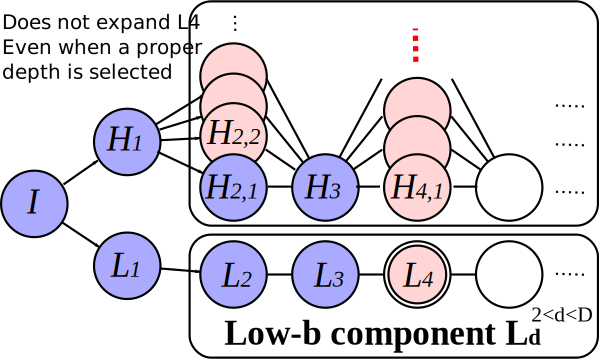
\includegraphics[width=0.49\linewidth]{img/model/rd2.pdf}
 \caption{$\fifo,\lifo,\ro,\depth$ all exhibit a pathological behavior due to the large number of successors and the large depth.}
 \label{fig:model-pathological}
\end{figure}

Consider a blind search on the directed acyclic graph
shown in \refig{fig:model}.
The graph consists of two large components, \textbf{high-b} and \textbf{low-b} branches, and their entries $H_1,L_1$. The initial search node is $I$ and the goal node is $L_4$.
Both branches have maximum depth $D$, and the high-b branch has maximum width $B$.
Both $B$ and $D$ are very large.
This graph presents a pathological case for all of the previously described methods (\lifo, \fifo, \ro and type-based diversification), depending on successor ordering.
\lifo performs a DFS, and if \lifo first searches $H_1$ and the high-b branch due to successor ordering, it must explore the entire high-b branch before expanding $L_1$ and low-b branch.
\fifo performs Breadth-First Search (BreadthFS), and  will therefore suffer from the  high branching factor at depth 2 of the high-b branch, getting stuck before reaching $L_4$.
Although randomization can allow \ro to be better off than the behavior of \fifo/BreadthFS, the effect is limited:
For example, while expanding depth 2, \ro may occasionally expand depth 3 because it uniformly randomly selects a node from OPEN.
However, the probability of expanding nodes at depth 3 is initially only $1/(B+1)$ and continues to be small until  most of the nodes at depth 2 are expanded, 
because OPEN is mostly populated with the nodes from depth 2.
Depth-based diversification addresses the depth bias of BreadthFS.
However, even though it distributes the effort among various depths,
the probability of expanding $L_2,L_4$ at depths 2 and 4, is only $1/(B+1)$ each, which is very low when $B$ is very large.

We propose \;\emph{Invasion Percolation-based diversification (IP-diversification)}, a new diversification strategy for satisficing search that addresses this type of bias.
% in \refig{fig:model} for satisficing planning,%not limited to planning
% As discussed above, a diversification scheme seeks to allocate resources evenly among a group of nodes in order to avoid undesirable biases.
% One approach to implementing diversification is to treat diversification in a search graph as the problem of evenly covering the graph over time.
% By considering the graph as a multidimensional lattice, we can apply techniques that have been developed for modeling percolation in multidimensional lattices.
IP-diversification combines randomization and Prim's method \cite{prim1957shortest} for Minimum Spanning Tree (MST).
% -- we seek an unbiased method for evenly exploring a search graph based on this model.

\section{Preliminaries and Definitions}

We first define some notation and the terminology used throughout the
rest of the paper.
$h(s)$ denotes the heuristic estimate from the current state $s$ to some
goal state.
$g(s)$ is the current shortest path cost from the initial state to the
current state.
$f(s)=g(s)+h(s)$ is the estimate of the resulting cost of the path
containing the current state.
We omit the argument $(s)$ unless necessary.

A \emph{sorting strategy} of a best first search algorithm is a strategy
which tries to select a single node from the OPEN list.
Each sorting strategy is denoted as a vector of several sorting
criteria, such as
[$\text{criterion}_1$, $\text{criterion}_2$, $\ldots$,
$\text{criterion}_k$], which means: From the OPEN list, first, select a
set of nodes using $\text{criterion}_1$.  If there are still multiple
nodes remaining in the set, then break ties using $\text{criterion}_2$
and so on, until a single node is selected.  The \emph{first-level
sorting policy} of a strategy is $\text{criterion}_1$, the
\emph{second-level sorting policy} is $\text{criterion}_2$, and so on.
%% the word frontier is no longer used in the later text.
% \emph{final frontier} is the set of open nodes with $f^*$.
Note that this corresponds to the command line option format of Fast
Downward \cite{Helmert2006}.

Using this notation, \astar without any tiebreaking strategy can be
denoted as a Best-First Search (BFS) with $[f]$, and \astar which breaks ties according to $h$
value is denoted as $[f,h]$. Similarly, GBFS is denoted as 
$[h]$.  Unless stated otherwise, we assume the nodes are sorted in the
increasing order of the key value, and a BFS always selects the smallest
key value.

The sorting strategy may fail to select a single node because some nodes
may share the same sorting keys. In such cases, a search algorithm must
decide which node to expand by a \emph{last-resort} tiebreaking
strategy, which is one of FIFO (First-In-First-Out), LIFO
(Last-In-First-Out) or RO (random ordering).  Trivially, these
strategies are able to select a single node from the set of
nodes. Although these last-resort strategies may not be a ``sorting''
criteria, we also include those strategies in the vector notation. For
example, an \astar using \fifo tiebreaking is denoted as $[f,h,\fifo]$.


A \emph{plateau} is a set of nodes in OPEN, the element of which are
indistinguishable according to the sorting strategy. In case of \astar
using tiebreaking with $h$ ($[f,h]$), this is the set of nodes with the
same $f$ cost and the same $h$ cost.
A plateau whose nodes have $f=f_p$ and $h=h_p$ is denoted as $\plateau{f_p,h_p}$.

An \emph{entrance} to a $\plateau{f_p,h_p}$ is a node $n \in
\plateau{f_p,h_p}$, whose current parent is not a member of
$\plateau{f_p,h_p}$.  The \emph{final plateau}, is the plateau
containing the solution found by the search algorithm.  In \astar using
admissible heuristics, the final plateau is $\plateau{f^*}$ (without
tiebreaking), or $\plateau{f^*,0}$ (with $h$-based tiebreaking).

\section{Background: Tiebreaking Strategies for \astar}

\label{sec:astar-background}

\astar is a standard search algorithm for finding an optimal-cost path
on a graph.
Starting from the single initial node, in each iteration, \astar
selects and expands a node $n$ with the lowest $f$-cost in the OPEN
priority queue. The successor nodes are inserted back to OPEN, and $n$
is marked as CLOSED, in order to avoid duplicated evaluations.
\astar returns an optimal solution when $h$ is admissible, i.e., when
$h(n) \leq h^*(n)$, where $h^*(n)$ is the optimal distance from $n$ to
the nearest goal.

The best-first order of the expansion is a key to guarantee solution optimality. 
The first solution found by the algorithm is guaranteed to have the optimal cost $f=f^*$ because 
all nodes with $f(n) < k$ are already expanded when it starts expanding
the nodes with $f(n) = k$.
Thus, the \emph{effective search space of \astar} is the set of nodes with 
$f(n) \leq f^*$: \astar expands all nodes with $f(n) < f^*$, then
expands \emph{some} of the nodes with $f(n) = f^*$, and
never expands a node with $f(n) > f^*$.

If multiple nodes with the same $f$-cost are possible, \astar
must implement some tiebreaking policy (either
explicitly or implicitly) which selects from among these nodes.
The early literature on heuristic search seems to have been mostly agnostic regarding tiebreaking.
The original \astar paper, as well as Nilsson's subsequent textbook 
states: ``Select the open node $n$ whose value $f$
is smallest. Resolve ties arbitrarily, but always in favor of any [goal
node]'' \cite[p.102 Step 2]{hart1968formal}, \cite[p.69]{Nilsson71}.
% Although it is possible to interpret this to imply $h$-based tiebreaking
% since goal nodes are the special case where $h=0$,
% they make no further mention of tiebreaking.
Pearl's textbook on heuristic search specifies that best-first search should ``break ties arbitrarily'' (\citeyear{pearl1984heuristics}, p.48, Step 3), and does not specifically mention tiebreaking for \astar.
To the best of our knowledge, the first explicit mention of a tiebreaking policy that considers node generation order is by Korf in his analysis of IDA*: ``If \astar employs the tiebreaking rule of 'most-recently generated', it must also expand the same nodes [as IDA*]'', i.e., a \lifo ordering.

In recent years, tiebreaking according to $h$-values has become ``folklore'' in the search community.
\citeauthor{hansen2007anytime} state that ``[i]t is well-known 
that \astar achieves best performance when it breaks ties
in favor of nodes with least h-cost'' \cite{hansen2007anytime}.
\citeauthor{holte2010common} writes ``\astar breaks ties in favor
of larger $g$-values, as is most often done'' \cite[note that since $f=g+h$,
preferring large $g$ is equivalent to preferring smaller $h$]{holte2010common}.
\shortciteauthor{felner2011inconsistent} also assume ``ties are broken in
favor of low h-values'' in describing Bidirectional Pathmax for \astar \citeyear{felner2011inconsistent}.
In their detailed survey/tutorial on efficient \astar implementations,
\shortciteauthor{burns2012implementing} \citeyear{burns2012implementing}
also break ties ``preferring high $g$'' (equivalent to low $h$).
%% this could be moved to later analysis
% They further write: ``The reasoning is that the goal can be found more
% quickly in the final $f$ layer of search''.
Thus, tiebreaking according to $h$-values appears
to be ubiquitous in practice while,
to our knowledge, an in-depth experimental analysis of tiebreaking strategies for \astar is lacking in the literature.

Although the standard practice of tiebreaking according to $h$ might be
sufficient in some domains, further levels of tiebreaking (explicit or
implicit) are required if multiple nodes have the same $f$ as well as
the same $h$ values. To date, the effect of such \emph{last-resort}
tiebreaking was not investigated in depth.
% 
For example, the survey of efficient \astar implementation techniques in
\cite{burns2012implementing} did not explicitly mention the last-resort
tiebreaking, while their library
code\footnote{https://github.com/eaburns/search} uses \lifo
last-resort tiebreaking.
% 
It first breaks ties according to $h$, and then
breaks remaining ties according to a \lifo policy (most recently
generated nodes first), i.e., $[f,h,\lifo]$.
% 
Although not documented, their choice of a \lifo 2nd-level tiebreaking
policy appears to be a natural consequence of the fact it can be
trivially, efficiently implemented in their two-level bucket (vector)
implementation of OPEN.
% 
In contrast, the current implementation of the \sota \astar based planner Fast
Downward \cite{Helmert2006}, as well as the work by \cite{RogerH10} uses
a $[f,h,\fifo]$ tiebreaking strategy.
% 
Although we could not find an explanation in the publication nor in the
website, this choice is most likely due to their use of alternating OPEN
lists, in which case the \fifo second-level policy serves to provide a
limited form of fairness.
% 
Such lack of explanation suggests that this topic has long been out
of focus of the heuristic search literature.

\section{Anatomy of Standard Strategies}
\label{sec:eval-common-strategies}

In order to construct new baselines and their performance differences,
we evaluated tiebreaking strategies for domain-independent optimal
classical planning.  In our experiments, all planners are based on Fast
Downward, and all experiments are run with a 5-minute,
4GB memory limit for the search binary (FD translation/preprocessing
times are not included in the 5-minute limit).  All experiments were
conducted on Xeon E5410@2.33GHz CPUs. 

% following paragraph is added in order to avoid repeating the list of domains not
% included due to no coverage difference.
We used 1104 instances from 35 standard benchmark domains. These
instances are those originally included in the test suite of Fast
Downward planning system. In detail, they are: airport(50),
barman-opt11(20), blocks(35), cybersec(19), depot(22), driverlog(20),
elevators-opt11(20), floortile-opt11(20), freecell(80), grid(5),
gripper(20), hanoi(30), logistics00(28), miconic(150), mprime(35),
mystery(30), nomystery-opt11(20), openstacks-opt11(20),
parcprinter-opt11(20), parking-opt11(20), pathways(30),
pegsol-opt11(20), pipesworld-notankage(50), pipesworld-tankage(50),
psr-small(50), rovers(40), scanalyzer-opt11(20), sokoban-opt11(20),
storage(30), tidybot-opt11(20), tpp(30), transport-opt11(20),
visitall-opt11(20), woodworking-opt11(20), zenotravel(20).

\subsection{Does Last-Resort Strategies Make a Difference?}

We first compared two commonly used tiebreaking strategies, $[f,h,\fifo]$, $[f,h,\lifo]$, which
first break ties according to $h$, and then apply \fifo or \lifo
last-resort tiebreaking, respectively.
Results for LMcut heuristic \cite{Helmert2009} and M\&S heuristic \cite{HelmertHHN14} are
shown in \reftbl{tbl:lmcut-ipc-std} and \reftbl{tbl:mands-ipc-std}
(leftmost 2 columns), respectively.
Differences in coverage are observed in several domains, and
$[f,h,\lifo]$ outperforms $[f,h,\fifo]$ overall.

\begin{table}[htbp]
 {
 \centering
 \begin{center}
\begin{tabular}{|l|cc|}
Sorting Criteria & IPC(1104) & IPC(1104)\\
 & \lmcut & \mands\\
 &  & \\
\([f,\fifo]\) & 443 & 460\\
\([f,\lifo]\) & 558 & 490\\
 &  & \\
\([f,h,\fifo]\) & 558 & 491\\
\([f,h,\lifo]\) & \textbf{565} & \textbf{496}\\
\end{tabular}
\end{center}

 \caption{
 Summary results: Coverage comparison (the number of instances solved in 5min, 4GB, LMcut
 heuristics) between
 the standard baseline tiebreaking algorithms. 
 }
 \label{tbl:lmcut-ipc-std}
 }
\end{table}


\begin{table}[htbp]
 {
 \centering
 \begin{center}
\begin{tabular}{|r|*{2}{ccc|}}
Domain & $[f,\fifo]$ & $[f,\lifo]$ & $[f,\ro]$ & $[f,h,\fifo]$ & $[f,h,\lifo]$ & $[f,h,\ro]$\\
IPC benchmark (1104) & 443 & 558 & 448.9 $\pm$ 1.3 & 558 & \textbf{565} & 558.9 $\pm$ 2.1\\
airport(50) & 18 & 26 & 18 $\pm$ 0 & \textbf{27} & 26 & 25.7 $\pm$ 0.5\\
barman-opt11(20) & 0 & 0 & 0 $\pm$ 0 & 0 & 0 & 0 $\pm$ 0\\
blocks(35) & 26 & 26 & 26 $\pm$ 0 & \textbf{28} & \textbf{28} & \textbf{28} $\pm$ 0\\
\textbf{cybersec(19)} & 0 & 3 & 0 $\pm$ 0 & 2 & 3 & \textbf{3.9} $\pm$ 1.1\\
depot(22) & 5 & 5 & 5 $\pm$ 0 & 6 & 6 & 6 $\pm$ 0\\
driverlog(20) & 12 & 13 & 12 $\pm$ 0 & 13 & 13 & 13 $\pm$ 0\\
elevators-opt11(20) & 14 & 15 & 14 $\pm$ 0 & 15 & 15 & 15 $\pm$ 0\\
floortile-opt11(20) & 6 & 6 & 6 $\pm$ 0 & 6 & 6 & 6 $\pm$ 0\\
freecell(80) & 8 & 9 & 8.7 $\pm$ 0.5 & 9 & 9 & 9 $\pm$ 0\\
grid(5) & 1 & 1 & 1 $\pm$ 0 & 1 & 1 & 1 $\pm$ 0\\
gripper(20) & 6 & 6 & 6 $\pm$ 0 & 6 & 6 & 6 $\pm$ 0\\
hanoi(30) & 12 & 12 & 12 $\pm$ 0 & 12 & 12 & 12 $\pm$ 0\\
logistics00(28) & 16 & 18 & 16 $\pm$ 0 & \textbf{20} & \textbf{20} & \textbf{20} $\pm$ 0\\
miconic(150) & 68 & 140 & 68 $\pm$ 0 & 140 & 140 & 140 $\pm$ 0\\
mprime(35) & 20 & \textbf{22} & 19.9 $\pm$ 0.3 & 21 & 21 & 20.9 $\pm$ 0.3\\
mystery(30) & 15 & 16 & 15 $\pm$ 0 & 16 & 16 & 15.2 $\pm$ 0.4\\
nomystery-opt11(20) & 12 & 13 & 12 $\pm$ 0 & \textbf{14} & \textbf{14} & \textbf{14} $\pm$ 0\\
\textbf{openstacks-opt11(20)} & 11 & \textbf{18} & 11.2 $\pm$ 0.4 & 11 & \textbf{18} & 11.7 $\pm$ 0.5\\
parcprinter-opt11(20) & 12 & 13 & 12 $\pm$ 0 & 13 & 13 & 13 $\pm$ 0\\
parking-opt11(20) & 1 & 1 & 1 $\pm$ 0 & 1 & 1 & 1 $\pm$ 0\\
pathways(30) & 4 & 5 & 4 $\pm$ 0 & 5 & 5 & 5 $\pm$ 0\\
pegsol-opt11(20) & 17 & 17 & 17 $\pm$ 0 & 17 & 17 & 17 $\pm$ 0\\
pipesworld-notankage(50) & 13 & 13 & 13 $\pm$ 0 & 14 & 14 & 14.6 $\pm$ 0.5\\
pipesworld-tankage(50) & 7 & 8 & 8 $\pm$ 0 & 8 & 8 & 8 $\pm$ 0\\
psr-small(50) & 48 & 48 & 48 $\pm$ 0 & 48 & 48 & 48 $\pm$ 0\\
rovers(40) & 7 & 7 & 7 $\pm$ 0 & 7 & 7 & 7 $\pm$ 0\\
scanalyzer-opt11(20) & 4 & \textbf{10} & 5.4 $\pm$ 0.7 & \textbf{10} & \textbf{10} & \textbf{10} $\pm$ 0\\
sokoban-opt11(20) & 19 & 19 & 19 $\pm$ 0 & 19 & 19 & 19 $\pm$ 0\\
storage(30) & 14 & 14 & 14 $\pm$ 0 & 14 & 14 & 14 $\pm$ 0\\
tidybot-opt11(20) & 11 & 12 & 11 $\pm$ 0 & 12 & 12 & 12 $\pm$ 0\\
tpp(30) & 6 & 6 & 6 $\pm$ 0 & 6 & 6 & 6 $\pm$ 0\\
transport-opt11(20) & 6 & 6 & 6 $\pm$ 0 & 6 & 6 & 6 $\pm$ 0\\
visitall-opt11(20) & 9 & 10 & 9.4 $\pm$ 0.5 & 10 & 10 & 10 $\pm$ 0\\
woodworking-opt11(20) & 6 & 9 & 8.2 $\pm$ 0.4 & \textbf{10} & \textbf{10} & \textbf{10} $\pm$ 0\\
zenotravel(20) & 9 & \textbf{11} & 9 $\pm$ 0 & \textbf{11} & \textbf{11} & \textbf{11} $\pm$ 0\\
\end{tabular}
\end{center}

 \caption{
 Coverage comparison (the number of instances solved in 5min, 4GB, LMcut
 heuristics) between
 the standard baseline tiebreaking algorithms. We highlight the
 best results when the difference between the maximum and the minimum coverage exceeds 2.
 }
 \label{tbl:lmcut-ipc-std}
 }
\end{table}

\begin{table}[htbp]
 {
 \centering
 \begin{center}
\begin{tabular}{|r|*{2}{ccc|}}
Domain & $[f,\fifo]$ & $[f,\lifo]$ & $[f,\ro]$ & $[f,h,\fifo]$ & $[f,h,\lifo]$ & $[f,h,\ro]$\\
IPC benchmark (1104) & 460 & 490 & 460.9 $\pm$ 1.6 & 491 & \textbf{496} & 489.4 $\pm$ 1.0\\
airport(50) & 9 & 9 & 9 $\pm$ 0 & 9 & 9 & 9 $\pm$ 0\\
barman-opt11(20) & 4 & 4 & 4 $\pm$ 0 & 4 & 4 & 4 $\pm$ 0\\
blocks(35) & 21 & 22 & 21 $\pm$ 0 & 22 & 22 & 22 $\pm$ 0\\
\textbf{cybersec(19)} & 0 & 0 & 0 $\pm$ 0 & 0 & 0 & 0 $\pm$ 0\\
depot(22) & 5 & 6 & 5 $\pm$ 0 & 6 & 6 & 5 $\pm$ 0\\
driverlog(20) & 12 & 12 & 12 $\pm$ 0 & 12 & 12 & 12 $\pm$ 0\\
elevators-opt11(20) & 13 & 13 & 13 $\pm$ 0 & 13 & 13 & 13 $\pm$ 0\\
floortile-opt11(20) & 5 & 6 & 5 $\pm$ 0 & 6 & 6 & 6 $\pm$ 0\\
freecell(80) & 15 & 16 & 15 $\pm$ 0 & \textbf{17} & \textbf{17} & 16 $\pm$ 0\\
grid(5) & 2 & 2 & 2 $\pm$ 0 & 2 & 2 & 2 $\pm$ 0\\
gripper(20) & 8 & \textbf{20} & 8 $\pm$ 0 & \textbf{20} & \textbf{20} & \textbf{20} $\pm$ 0\\
hanoi(30) & 14 & 14 & 14 $\pm$ 0 & 14 & 14 & 14 $\pm$ 0\\
logistics00(28) & 20 & 20 & 20 $\pm$ 0 & 20 & 20 & 20 $\pm$ 0\\
miconic(150) & 68 & \textbf{73} & 68.3 $\pm$ 0.7 & \textbf{73} & \textbf{73} & \textbf{73.2} $\pm$ 0.4\\
mprime(35) & 23 & 23 & 22 $\pm$ 0 & 23 & \textbf{24} & 23.7 $\pm$ 0.5\\
mystery(30) & 15 & 15 & 15 $\pm$ 0 & 15 & 16 & 15 $\pm$ 0\\
nomystery-opt11(20) & 17 & 18 & 17.8 $\pm$ 0.4 & 18 & 18 & 18 $\pm$ 0\\
\textbf{openstacks-opt11(20)} & 15 & \textbf{19} & 15.4 $\pm$ 0.5 & 15 & \textbf{19} & 15.4 $\pm$ 0.5\\
parcprinter-opt11(20) & 10 & 10 & 10 $\pm$ 0 & 10 & 10 & 10 $\pm$ 0\\
parking-opt11(20) & 1 & 1 & 1 $\pm$ 0 & 1 & 1 & 1 $\pm$ 0\\
pathways(30) & 4 & 4 & 4 $\pm$ 0 & 4 & 4 & 4 $\pm$ 0\\
pegsol-opt11(20) & 17 & \textbf{19} & 17.2 $\pm$ 0.4 & \textbf{19} & \textbf{19} & \textbf{19} $\pm$ 0\\
pipesworld-notankage(50) & 9 & 9 & 8.9 $\pm$ 0.3 & 10 & 10 & 9.9 $\pm$ 0.3\\
pipesworld-tankage(50) & 13 & 13 & 13.1 $\pm$ 0.3 & 13 & 13 & 13.2 $\pm$ 0.4\\
psr-small(50) & 50 & 50 & 50 $\pm$ 0 & 50 & 50 & 50 $\pm$ 0\\
rovers(40) & 6 & \textbf{8} & 6.1 $\pm$ 0.3 & \textbf{8} & \textbf{8} & \textbf{8} $\pm$ 0\\
scanalyzer-opt11(20) & 10 & 10 & 10 $\pm$ 0 & 10 & 10 & 10 $\pm$ 0\\
sokoban-opt11(20) & 20 & 20 & 20 $\pm$ 0 & 20 & 20 & 20 $\pm$ 0\\
storage(30) & 15 & 15 & 15 $\pm$ 0 & 15 & 15 & 15 $\pm$ 0\\
tidybot-opt11(20) & 0 & 0 & 0 $\pm$ 0 & 0 & 0 & 0 $\pm$ 0\\
tpp(30) & 6 & 6 & 6 $\pm$ 0 & 7 & 6 & 6 $\pm$ 0\\
transport-opt11(20) & 7 & 7 & 7 $\pm$ 0 & 7 & 7 & 7 $\pm$ 0\\
visitall-opt11(20) & 9 & 9 & 9 $\pm$ 0 & 9 & 9 & 9 $\pm$ 0\\
woodworking-opt11(20) & 7 & 7 & 7 $\pm$ 0 & 7 & 7 & 7 $\pm$ 0\\
zenotravel(20) & 10 & 10 & 10 $\pm$ 0 & \textbf{12} & \textbf{12} & \textbf{12} $\pm$ 0\\
\end{tabular}
\end{center}

 \caption{
 Coverage comparison (the number of instances solved in 5min, 4GB, M\&S heuristics) between
 the standard baseline tiebreaking algorithms. We highlight the
 best results when the difference between the maximum and the minimum coverage exceeds 2.
 }
 \label{tbl:mands-ipc-std}
 }
\end{table}

\subsection{Is $h$-Based Tiebreaking Necessary?}

\label{sec:noh}

In the right half of \reftbl{tbl:lmcut-ipc-std} and
\reftbl{tbl:mands-ipc-std}, we show the results of $[f, \fifo]$ and
$[f, \lifo]$, the \astar variants which rely on \fifo or \lifo
last-resort tiebreaking only.  $[f,\lifo]$, which simply breaks ties
among nodes with the same $f$-cost by expanding the most recently
generated nodes first \cite{korf1985depth}, clearly dominates
$[f,\fifo]$.  Interestingly, the performance of the $[f,\lifo]$ strategy
is comparable to $[f,h,\lifo]$ and $[f,h,\fifo]$.
This may be surprising, considering the ubiquity of $h$-based tiebreaking in the search and planning communities.

\lifo behaves somewhat similarly to $h$-based tiebreaking, in the following sense:
\lifo expands the most recently generated node $n$.
For any child $n'$, 
if the heuristic function is admissible and $f(n') = f(n)$, there are only 2 possibilities :
(1) $g(n') > g(n)$ and $h(n') < h(n)$, or
(2) $g(n') = g(n)$ and $h(n') = h(n)$,
because $g(n)+h(n)=g(n')+h(n')$.
Thus, as \lifo expands nodes in a ``depth-first'' manner,
the nodes that continue to be expanded in the plateau by \lifo have non-increasing $h$-values,
much like in $h$-based tiebreaking which always searches toward the least $h$ cost.
Although the expansion order of $[f,\lifo]$ is not strictly the same as that of $h$-based tiebreaking strategies,
this explains their similarity in performances.

% \textbf{An in-depth investigation of the behavior of $[f,\lifo]$ vs. $h$-based tiebreaking is a direction for future work.}
% Compared to the $h$-based variants which explicitly selects nodes with smaller $h$ and its expanded nodes have non-increasing $h$-values,
% This has the same  can behave somewhat similarly to actively expanding nodes with low $h$-values, as done by $h$-based tiebreaking.
% \citeauthor{burns2012implementing}
% (\citeyear{burns2012implementing}) writes ``the goal can be found more
% quickly in the final $f$ layer of search'' about $h$ tiebreaking.

\subsection{Plateaus and Tiebreaking}

\refig{fig:f-h-eval} gives us a
more fine-grained analysis by comparing the number of node evaluation
(computations of \lmcut) in each instance between $[f,h,\lifo]$ and $[f,h,\fifo]$ strategies.
It shows that the difference in the number of nodes
evaluated can sometimes be larger than a factor of 10 (\pddl{Openstacks}, \pddl{Cybersec} domains).
Contrary to the conventional wisdom, 
these results suggest that last-resort tiebreaking can have a significant effect on
the search performance.

\begin{figure}[htbp]
 \centering \relsize{-3}
 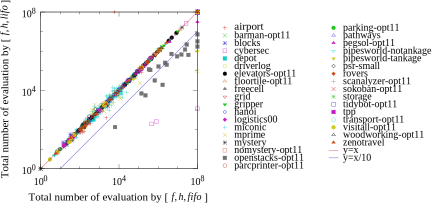
\includegraphics{tables/aaai16-30min-5min-cut/aaai16prelim3/evaluated-lmcut_ff-lmcut_lf.pdf}
 \caption{The number of LMcut evaluations on various planning domains,
 with standard \fifo vs \lifo last-resort tiebreaking, both with $h$
 tiebreaking. \lifo evaluates  less than $1/10$ of the nodes evaluated
 by \fifo in \pddl{Cybersec} and \pddl{Openstacks}. 
 }
 \label{fig:f-h-eval}
\end{figure}

% In a plateau, the heuristics do not provide any useful guidance -- a
% plateau region requires a blind search because all neighboring nodes have the same
% estimates. Because of this, search algorithms rely solely on the tiebreaking criterion.

% We further investigate the cause of this performance difference in detail.

The effect of the last-resort tiebreaking strategies (\lifo or
\fifo) under the presence of $h$-tiebreaking is
limited to the search plateau $\plateau{f,h}$, the set of nodes which
share the same $f$ values and $h$ values.
% 
Also, in optimal search, the two \astar with
different last-resort tiebreaking strategies both search the same set of
nodes in the region where $f<f^*$.
% 
% If $h$-tiebreaking is enabled, the two \astar variants also expands the same number of nodes with $h>0$.
Furthermore, the nodes with $h>0$ never become the goal nodes when $h$ is admissible.
% 
Therefore, the effect of last-resort tiebreaking is limited to
the final plateau $\plateau{f^*,0}$.
 
Conventionally, 
this final plateau, $\plateau{f^*,0}$, was naively considered to be very small compared to the
total size of the search space required to be expanded by \astar.
However, counter-intuitively, such a region can be so large enough to
cause a performance difference, or in fact it can even account for \emph{most} of the
search effort required by \astar.

\refig{fig:plateau} plots the size of this final plateau on 1104 IPC
benchmark instances.  The $y$-axis represents the number of nodes with
$f=f^*, h=0$, the final plateau, and the $x$-axis represents the total
number of nodes expanded so far. This figure suggests that, in some
domains such as \pddl{Openstacks} and \pddl{Cybersec}, the planner
spends most of the runtime searching the final plateau for a solution,
even with the help of $h$ tiebreaking.

One natural question might be about what makes these two domains,
\pddl{Openstacks} and \pddl{Cybersec}, different from all other domains
which have much smaller final plateaus.

\begin{figure}[htbp]
   \centering
  \includegraphics{tables/aaai16-frontier/aaai16prelim3/lmcut_frontier-front.pdf}
  \caption{
 The number of nodes with $f=f^*, h=0$ (y-axis), which form
  the final plateau when $h$-based tiebreaking is enabled, compared to
  the total number of nodes in the search space (x-axis) with $f\leq
  f^*$ on 1104 IPC benchmark problems.  Note that \pddl{Openstacks}
  and \pddl{Cybersec} instances are near the $y=x$ line.
  This statistics is obtained by running a modified Fast Downward with
 \lmcut which continues searching after the solution is found
 until expanding all nodes with cost $f=f^*$.} \label{fig:plateau}
\end{figure}


\section{Domains with Zero-Cost Actions}
\label{sec:zerocost-domains}
%% best to put openstacks here, considering the connection to the
%% previous section
\pddl{Openstacks}  is a cost
minimization domain introduced in IPC-2006, where the objective is to 
minimize the number of stacks used.
There are many zero-cost actions (i.e., actions that don't increase the number of stacks), and
they prevent the standard heuristics from producing
informative guidance.

%% safe to remove these explanation.
% According to \cite{richter2010lama}, \textbf{??????}
% %Richter talks about the failures on openstacks starting around p.167
% \lmcut \cite{Helmert2009} fails to find a good cost
% partitioning with non-zero values, 
% % A detailed discussion of Openstacks domain and poor performance of landmarks is in \cite{richter10lama}, p.167-169.
% and most edges in the abstraction
% space of M\&S \cite{helmert2007flexible} have zero costs.


% XXX I'm commenting out the paragraphs below because:
% (1) A review of heuristic functions for domain-independent learning is not really
% necessary for this AAAI submission. 
% (2) It's better if this paper is not so strongly associated with the ICAPS community only -- this work applies in general to search with A*, and is not strongly tied to almost-perfect heuristics, lmcut, m&s, etc.

Although domains with zero-cost actions are not common in the current set of benchmarks, we argue that such domains are of an important class of models for cost-minimization problems, i.e.,
assigning zero costs make sense from a practical, modeling perspective.
For example, consider the \pddl{driverlog} domain, where the task is to move packages between locations using trucks.
The IPC version of this domain assigns unit costs to all actions. Thus, cost-optimal planning on this domain seeks to minimize the number of steps in the plan.
However, another natural objective function would be the one which minimizes the amount of fuel spent by driving the trucks,
assigning cost 0 to all actions except \pddl{drive-truck}.

% While I agree with the point you're trying to make,
% There is an ugly issue when arguing that current models try to  optimize plan-execution time (i.e., makespan), 
% which is that if we really cared about makespan optimality, we would consider parallel execution of actions whenever possible.
% however, sequential classical planners do not handle parallel actions at all  (recall ACP).
% so arguing this path can only lead to trouble.. Let's try a safer line of argument.
%% For runtime minimization,
%% nonzero positive costs are reasonable because
%% every actions are supposed to consume a fraction of time.
%% However, such formulation is not suitable for general optimization
%% problems.  For example, when you try to minimize the energy consumption
%% by the elevators in \pddl{Elevators} domain, many actions would have zero-cost
%% --- it does not consume electricity for either boarding or leaving the
%% passenger, or moving the elevator down.
%% % 
%% From the practical point of
%% view, cost minimization domains would have wider interest compared to
%% the simple runtime minimization.
%% Also, as shown previously, such domains pose a
%% difficulty to the current heuristic planners due to their large plateaus.

Similarly, for many practical applications, a natural objective is to
optimize the usage of one key consumable resource, e.g., fuel/energy
minimization.  In fact, two of the IPC domains, \pddl{Openstacks} and
\pddl{Cybersec}, which were shown difficult for standard tiebreaking
methods in the previous section, both contain many zero-cost actions,
and \textbf{both are based on industrial applications}: \pddl{Openstacks} models
production planning \cite{fink1999applications} and \pddl{Cybersec}
models Behavioral Adversary Modeling System \cite[minimizing decryption,
data transfer, etc.]{boddy2005course}.

Therefore, in this paper, we modified various domains
into cost minimization domains with many zero-cost actions.
Specifically, a domain is modified so that all action schemas are assigned
cost 0 except for a few (usually one) action schema which consumes some key resource.
The last word in the names of these domains indicate the action which is
assigned non-zero cost, e.g., \pddl{elevator-up} is a modified elevator
domain where the \pddl{up} action is assigned non-zero cost (because
elevators are considered to consume energy only when going \pddl{up}), and all other actions have cost 0.
Most of the transportation-type domains are modified to optimize 
energy usage (\pddl{Logistics-fuel}, \pddl{elevator-up} etc.), and  assembly-type domains are modified to minimize resource usage
%% floortile-ink is not shown, so better not to mention it
(\pddl{Woodworking-cut} minimizes wood usage, etc.).
We did not
include domains with only a single action schema and standard domains which already had many
zero-cost actions (these are already in the results for standard IPC domains).
We refer to these 28 new domains as \emph{zerocost domains}.

\refig{fig:plateau-zerocost} plots the size of the final plateau of the
zerocost domain instances, with $h$-tiebreaking enabled.  As expected,
many of these zerocost domains have large plateaus even with the help of
$h$-tiebreaking.  Thus, in these cost-minimization problems, the search
strategy within plateaus, i.e., tiebreaking, becomes a yet more critical
factor which determines the search performance.

\begin{figure}[htbp]
  \centering
  \includegraphics{tables/aaai16-frontier/zerocost/lmcut_frontier-front.pdf}
  \caption{Similar to \refig{fig:plateau}, but for 620 instances from our 
  \emph{zerocost domains} (\refsec{sec:zerocost-domains}),
  where zero-cost actions induce very large plateaus.
 }
 \label{fig:plateau-zerocost}
\end{figure}

Note that the difficulty posed by these domains sometimes \emph{cannot}
be tackled by improving the heuristic estimates, or reducing the
underestimation by an admissible heuristic function.  Due to the
existence of 0-cost edges, some non-goal nodes around a goal node can
legitimately have a distance to the goal equal to 0. For those nodes,
there are no means to improve the heuristic estimate to any positive
value without making the heuristics inadmissible, because it is
an overestimation.

Thus, in order to solve zerocost problems more efficiently, the planner
needs to perform an efficient \emph{knowledge-free} search within a
large, final plateau. It turns out that a notion of \emph{depth} can
have a significant impact on the performacne of knowledge-free search,
as well as a good understanding ot the existing tiebreaking strategies.

\section{Depth-Based Tiebreaking for A*}

\label{sec:depth}

In Zerocost domains, the search space has a lot of zero-cost edges,
producing a large final plateau $\plateau{f^*,0}$. In a final plateau,
all nodes have $h=0$ which inhibit the $h$-based tiebreaking to provide
a useful guidance toward a goal. Without adequate measure, search
algorithms may fail to keep track of the current search progress.

The \emph{depth} of a node is an instance of such measurement.  It is an
integer value representing the distance (number of steps) from the
\emph{entrance} of the plateau.  An \emph{entrance} of the plateau is
the first node which entered the plateau, along the path from the
initial node. These notions are depicted in
\refig{fig:plateau-depiction}. It is equivalent to the $g$-value which is
restricted to a particular plateau and is assuming the unit cost edges.

\begin{figure}[htbp]
 \centering
 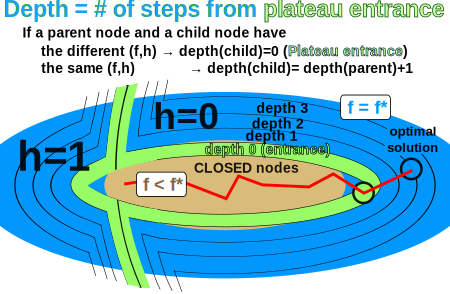
\includegraphics{img/astar/final-plateau4.png}
 \caption{The nodes in a platau are divided into several layers,
 and each layor have the corresponding depth.}
 \label{fig:plateau-depiction}
\end{figure}

The depth $d(n)$ of a
node $n$ is 0 when $n$ and the parent node $m$ has the different key
values for a sorting strategy, and $d(n)=d(m)+1$ when they have the same
key values: For example, in \astar with $h$-based tiebreaking, the key
values of a node are represented as a vector $[f,h]$, and they are same
when they are pairwise equivalent (i.e. $f(n) = f(m) \land h(n) =
h(m)$).  Having the same key values means that $n$ and $m$ are in the
same plateau. \todo{Figure}

The traditional \lifo and \fifo tiebreaking strategy are
searching the plateau region in a decreasing or increasing order of the depth.
\lifo strategy always selects the most recently generated node
within $\plateau{f,h}$, and the behavior in the plateau is equivalent to depth-first search.
Thus, it results in always selecting the largest depth
buckets as depicted in \refig{fig:plateau-depiction-lifo}.
Similarly, the behavior of \fifo strategy 
in a plateau is equivalent to breadth-first search. Thus \fifo strategy
always selects the nodes with least depth (\refig{fig:plateau-depiction-fifo}).
Note that therefore $[f,h,\lifo]$ is equivalent to $[f,h,-d,\lifo]$ and
$[f,h,\fifo]$ is equivalent to $[f,h,d,\fifo]$.

\begin{figure}[htbp]
 \centering
 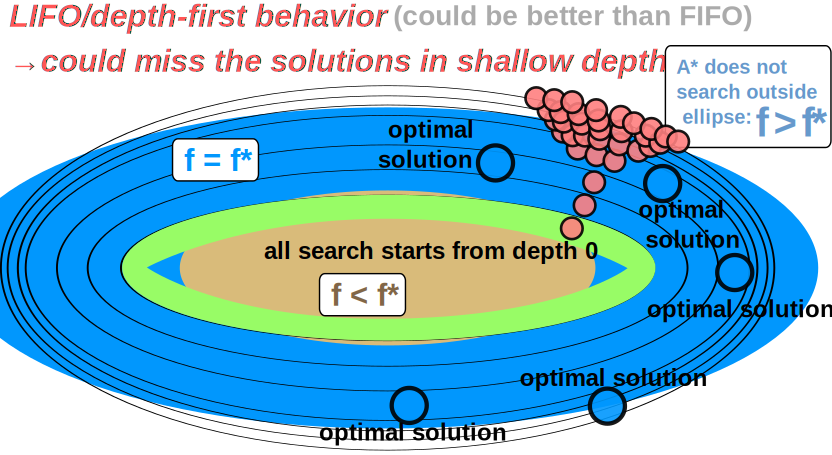
\includegraphics{img/astar/final-plateau6.png}
 \caption{\lifo tiebreaking strategy implies a depth-first behavior in a
 plateau, which could miss the solution concentrated near the entrance.}
 \label{fig:plateau-depiction-lifo}
\end{figure}

\begin{figure}[htbp]
 \centering
 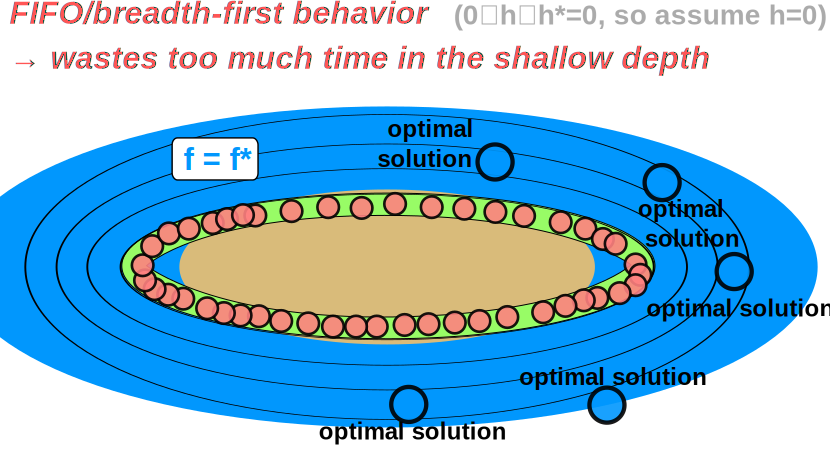
\includegraphics{img/astar/final-plateau5.png}
 \caption{\fifo tiebreaking strategy implies a breadth-first behavior in a
 plateau, which could fail to reach a solution in the deeper region
 within the time limit.}
 \label{fig:plateau-depiction-fifo}
\end{figure}

The problem in these traditional strategies is that we have no knowledge
on whether the goals are located near or far from the entrance. Remind
that since $f=f^*, h=h^*=0$, any goals in this plateau are optimal
regardless of the depth: A goal node in a shallower region or a deeper
region both yields a cost-optimal solution. However, until we find a
solution, we do not know how the goals are distributed among various
depths. In some problem instance the goals can be concentrated around
the entrance, and in another problem instance the goals can be
concentrated in some large depth $k$.

% \begin{figure}[htbp]
%  \includegraphics{img/astar/final-plateau4-2.png}
%  \label{fig:plateau-depiction-all-optimal}
% \end{figure}

The best-first search (\fifo), which naturally focuses the search around
the entrance favoring the smaller depths, should perform better in the
former case, while it also severely degrade the performance in the
latter case because it searches the
shallower region exhaustively and takes too much time to reach the depth
where the goals exist.
Exactly the opposite could happen to depth-first search (\lifo):
\lifo greedily explores the
plateau region and may find a solution in the deeper region quickly but
could also miss the solution in the shallower region.
Thus, both \fifo and \lifo tiebreaking have pathological behaviors.

By an adversary argument, we propose a depth-based \emph{diversification}
tiebreaking strategy, which diversify the search among various depths.
Its search behavior is not biased toward any particular direction and
does not exhibit the pathological behavior.

In this strategy, the nodes are inserted into buckets
associated with depths, and upon expansion, search effort is distributed
among various depths. Notice that it does not ``sort'' the nodes
according to the increasing or decreasing order of depth,
and instead ``diversify'' the node expansion
within the plateau. We mark such a diversification family of
tiebreaking strategies by enclosing it in brackets such as $[f,h,\depth]$.

In order to diversify the expansion among depths, we propose simply
iterating over the depth buckets. There is a counter $d_c$ initialized
to 0, which stores the depth which was selected in the last expansion.
In each expansion, it decrements the counter ($d_c\leftarrow d_c-1$) and
expands from the bucket of $d_c$. When $d_c$ reaches below 0, then $d_c$
is reset to the current largest depth in the plateau.
It is possible to adopt a
nondeterministic, randomized selection, as we have done in a conference
version of this paper, however we eliminate the possibility of the
results being affected by random seeds. It also makes a theoretical
analysis more convenient in the later section.

\begin{figure}[htbp]
 \centering
 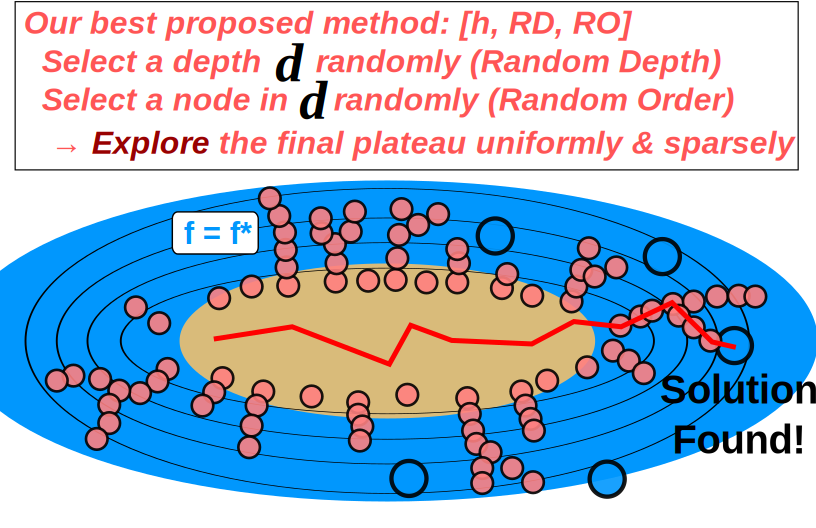
\includegraphics{img/astar/final-plateau7.png}
 \caption{Depth-based diversification allows \astar to search the plateau space
 uniformly and sparsely, avoiding the concentration to shallower depths, while
 suppressing the excessive exploration to the deeper region. This
 balances the exploration and exploitation.}
 \label{fig:plateau-depiction-all-optimal}
\end{figure}

% We later show that
% \fifo and \lifo strategies are incomplete when the size of the plateau
% region is inifinite, while our \id is probabilistically complete.

\subsection{The Scope Captured by Depth-Based Tiebreaking}

Depth-based tiebreaking has no effect when the key values for measuring
the depth are always updated and thus all nodes have depth 0. A key
value is a single $f$ when $h$-based tiebreaking is not present, and a
pair of $f$ and $h$ when $h$-based tiebreaking is present. When all
nodes have depth 0, the search is equivalent to the case where 
the depth-based strategy is not present.
% 
This happens when the target problem contains
positive costs\footnote{not to be confused with non-negative cost} only.
Let a node $n$ is reached from a node $m$. Assume
 $g(n)>g(m)+c$ where $c$ is a positive edge cost, and the parent of $n$
 is updated to $m$.

\begin{itemize}
 \item 
       If $f(n)=f(m)$, $h(n)<h(m)$ should hold because the new value of
       $g(n)$ is $g(m)+c>g(m)$. Therefore the depth is 0.
 \item If $h$-value is unchanged and $g$ is increased due to a positive
       cost edge, then $f$ is also increased, thus the depth is 0.
\end{itemize}

One might wonder what if the evaluated nodes are already visited from
another parent (old parent) with smaller $g$ value, and the new $g$ value does not change it,
which may cause the new parent and the child node may have the same $f$ and
same $h$. It does not result in a positive depth because it does not update the parent. The depth of a
child remains the old value (using the old parent), which is 0.


\subsection{Tiebreaking within Depth Buckets}

Since there can be still multiple nodes within the same depth bucket, a
last-resort tiebreaking is still necessary to break ties among them.
We can, for example, apply \lifo, \fifo or \ro (random order) policies
at this level.

There could be still a room for heuristic-agnostic improvements at
this level, while this is not in the scope of this paper.
For example, while depth metric measures and diversifies the depth in a plateau,
other techniques can non-trivially diversify the search in a breadth direction.
Such techniques may include pruning techniques such as 
Symmetry Breaking \cite{Fox1998,pochter2011exploiting,domshlak2013symmetry}
or Partial Order Reduction \cite{hall2013faster,wehrle2013relative}.

While these methods are most often described as ``pruning techniques'',
it can be rephrased as ``removing the cardinality bias to particular set
of nodes which share the same characteristics'' because they both aim to
prune the redundant nodes. Note that redunduncy causes a biased 
search effort. For example, imagine we have a
set of nodes $S=\{a_1, a_2, a_3, a_4, b, c, d\}$ where
$A=\{a_1, a_2, a_3, a_4\}$ are ``redundunt'' in some measure (e.g. by Symmetry,
Partial-Order). 
If a search algorithm expands $S$ by random selection, it favors the
group $A$ by giving a 4 times larger chance of expansion than $b$,
$c$ or $d$.

% \todo{compare id,fifo and id,lifo}

% However we use a Random Order (\ro) policy, which 
% randomly selects an element from the depth bucket selected by the depth-based tiebreaking.
% This is because the effectiveness of the tiebreaking behavior within a bucket
% can be affected by accidental biases, e.g., names/orders of action schema in the PDDL domain
% definition \cite{vallati2015effective}.
% %Finding the best action ordering is not the scope of this paper.
% Thus, we avoid bias at this level of tiebreaking by using \ro and assess its expected/average
% performance.

% Among \fifo, \lifo and \ro, the natural policy is Random Order.
% This is because the effectiveness of the third-level tiebreaking behavior
% is affected by the accidental bias in action ordering in the PDDL domain
% definition.  Recent work \cite{vallati2015effective} showed that the
% planner performance is greatly affected by changing and tuning the action ordering
% (and also variable ordering, but it is irrelevant to the tiebreaking behavior). 
% However, finding the best third-level tiebreaking is not the scope of this paper.
% Thus, focusing on \ro and assess its expected/average
% performance is the most reasonable practice to understand the behavior of second-level,
% depth-based tiebreaking.

\subsection{Theoretical Characteristics of the Depth Distribution}

We give further insight into the search behavior of our implementation
of depth-based diversification.
As stated, our implementation iterates from the largest depth to 0.

We are particularly interested in how the expansions happen among the
various depths in the plateau region.
We show that the probability of expanding a node in a particular depth
can be represented by a simple formula.  Although the notion of
probability does not fit well with deterministic \fifo or \lifo
last-resort tiebreaking, it is meaningful in the case of \ro (random
order) last-resort tiebreaking.

%% danger!!
% \begin{theo}[Uniformness of the search]
%  Assume the search space forms a tree of fixed width $w\geq 2$.
%  After enough number of iterations $D$,
%  the chance of expanding each node is unaffected by the depth of the
%  node, if the depth $d$ is small relative to $D$.
% \end{theo}

% I no longer claim the distribution is uniform.
As a preparation, we first show that the number of expansion happened to each depth decreases
linearly to the depth.
% 
Assume that each depth bucket never exhausts as a result of
expansion.  If the expansion of a node in the largest depth $D\geq 0$ resulted
in more nodes in the same plateau, then the newly generated nodes have
depth $D+1$.  Also, as we explained in the previous section, the
expansion is diversified by a sequence of iterations from the current
largest depth to 0.  It means that when the current maximum depth of
the plateau is $D\geq 0$, the number of iteration happened so far is also $D$.
Therefore, at the end of the $D$'th iteration, each depth $d$ has
been expanded exactly $D-d$ times, meaning that the chance of
expanding each depth is decreasing as the depth increase.

% However, it does not mean that this strategy favors the nodes in the
% shallower region.
% This is because the number of nodes in each depth is
% exponential to $d$, which is common in practice (we verify this in the
% later experiments).
Now we show the formula which represents the probability of expanding a node in a particular depth.
We assume that the plateau region form a tree of width
$w\geq 2$, rather than a graph with indefinite number of successor
nodes.  Under this assumption, each expansion of depth $d$ results in
$w$ new nodes in depth $d+1$. Also, if there are initially
$D$ nodes in depth 0, each depth bucket never exhausts until the end of $D$'th
iteration (when depth 0 becomes empty).

% $D-d$th expansion in the $D$th iteration expands the depth $d$.
At the end of $D$th iteration,
each depth $d-1$ is expanded $D-(d-1)$ times in the preceeding $D$ iterations.
Therefore, the total number of nodes that have been in depth $d$, including those
that have been expanded so far, is $w(D-d+1)$.
Expansion has happened $D(D-1)$ times in total, and depth $d$ is expanded $D-d$ times.
Thus, the probability of expanding each node in depth $d$ is
$\frac{D-d}{D(D-1)\cdot w(D-d+1)}=\frac{1}{wD(D-1)}(1-\frac{1}{D-d+1})$.  \qed

Notice that $\frac{1}{D-d+1}$ is negligeble if $D \gg d$.
Thus, after enough number of iterations (large $D$), the nodes are 
expanded in an approximately equal probability $\frac{1}{wD(D-1)}$ in the shallower region, and is
unaffected by the depth of the node.
However, the nodes near the largest depth has less probability, showing
some balance in exploration and exploitation.

The important point of this characteristics is that this
distribution is maintained at any point of the search until the solution
is found. In fact, any depth-selection criteria, including the least
depth selection (\fifo) or the largest depth selection (\lifo), 
result in the same distribution if all nodes are to be expanded (each
depth $d$ is expanded $Dw^d$ times), but their
online characteristics are not.

\section{Evaluating Depth-Based Tie-Breaking}
\label{sec:depth-based-evaluation}

% this text is mostly repeated below, so deleted this and promoted the subsection below up 1 level.
%% We evaluated our depth-based diversifying tie-breaking strategies against standard
%% tie-breaking strategies.
%% In addition to the 35 IPC benchmark domains with 1104 instances used in
%% the previous set of experiments, we used 28 Zerocost domains with 620
%% instances.  

%\subsection{Evaluating Depth-Based Tie-Breaking with $h$ tie-breaking}

We compared the performance of standard tie-breaking methods to depth-based tie-breaking methods. These all use $h$
as the second-level sorting criterion and either \fifo, \lifo or \ro (random order) default tie-breaking criterion.
The only difference is the presence of the third, depth-diversification criterion.

Experiments are conducted on {1104 standard IPC benchmark
instances} from 35 domains  and {620 Zerocost instances} from 28 domains (see \refsec{sec:eval-common-strategies} and \refsec{sec:zerocost-domains} for full lists of these domains). 
The basic experimental settings are the same as the previous ones:
Each experiment uses the Fast Downward planner using \astar search and either the \lmcut heuristic or \mands heuristic.
Each experiment is run for 5 minutes excluding SAS translation time, with 4GB memory constraints.

We first show the summary results of these experiments (\reftbl{tbl:depth-summary}).
Overall, depth-based tie-breaking tends to show larger coverages than the
standard tie-breaking strategies.
Interestingly, when the depth diversity criterion $\depth$ is used, 
the performance relationship between \lifo and \fifo seems to flip:
\fifo tends to perform better than \lifo in Zerocost domains for both
\lmcut and \mands heuristics (299 vs 279 for \lmcut, 317 vs 303 for \mands).
Also, \ro (random order) outperforms both \fifo and \lifo.
In the following, we describe and discuss each experiment.
Detailed data tables are in the Appendix (\refsec{sec:appendix}).

\begin{table}[htb]
 {
 \centering
 \setlength{\tabcolsep}{3pt}
 \begin{center}
\begin{tabular}{|l|cc|cc|}
Sorting Criteria & Zerocost(620) & Zerocost(620) & IPC(1104) & IPC(1104)\\
 & \lmcut & \mands & \lmcut & \mands\\
Standard &  &  &  & \\
$[f,h,\fifo]$ & 256 & 280 & 558 & 491\\
$[f,h,\lifo]$ & 279 & 301 & 565 & \textbf{496}\\
$[f,h,\ro]$ & 261.9 $\pm$ 1.4 & 287.7 $\pm$ 3.2 & 558.9 $\pm$ 2.1 & 489.4 $\pm$ 1.0\\
 &  &  &  & \\
Depth-based &  &  &  & \\
$[f,h,\depth,\fifo]$ & 284 & 302 & 571 & 487\\
$[f,h,\depth,\lifo]$ & 264 & 288 & \textbf{575} & 487\\
$[f,h,\depth,\ro]$ & \textbf{288.1 $\pm$ 1.6} & \textbf{308.1 $\pm$ 2.1} & 571.4 $\pm$ 1.7 & 485.6 $\pm$ 1.5\\
\end{tabular}
\end{center}

 \caption{
 Main summary results: Coverage comparison (number of instances solved in 5min, 4GB, \lmcut/\mands
 heuristics) between standard tie-breaking and depth-based tie-breaking
 ($\depth$). When \lmcut is used, $\depth$ outperforms standard strategies both in IPC
 instances (1104 problems total) and Zerocost instances (620 problems
 total). When \mands is used, $\depth$ outperforms standard strategies
 in Zerocost instances. \textbf{Bold} shows the best configuration.}
 \label{tbl:depth-summary}
 }
\end{table}

\reftbl{tbl:lmcut-zerocost-full} and \reftbl{tbl:mands-zerocost-full} show the number of Zerocost
instances (out of 620) solved by \lmcut and \mands heuristics. In these
Zerocost domains, our proposed method outperforms the traditional tie-breaking methods in both heuristics.
Significant improvements were observed in 10 domains when using \lmcut, and 7 domains when using \mands.

%% Removed in order to reduce the paper length
% In detail,
% \begin{itemize}
%  \item \textbf{10 Domains improved by depth on Zerocost, using \lmcut,} are \pddl{elevators-up} (\ro), \pddl{freecell-move} (\fifo,\ro),
%        \pddl{miconic-up} (all), \pddl{mprime-succumb} (\fifo,\ro), \pddl{pipesnt-pushstart} (\ro), \pddl{pipesworld-pushend} (\ro),
%        \pddl{scanalyzer-analyze} (\lifo), \pddl{storage-lift} (\fifo), \pddl{tpp-fuel} (\fifo,\ro), \pddl{woodworking-cut} (\fifo,\ro).
%  \item \textbf{7 Domains improved by depth on Zerocost, using \mands,} are \pddl{elevators-up} (\ro), \pddl{freecell-move} (\fifo,\ro),
%        \pddl{mprime-succumb} (\fifo,\ro), \pddl{pipesnt-pushstart} (\fifo, \ro), \pddl{pipesworld-pushend} (\ro),
%        \pddl{tpp-fuel} (\fifo,\ro), \pddl{woodworking-cut} (\fifo,\ro).
% \end{itemize}

\reftbl{tbl:lmcut-ipc-full} shows the number standard IPC benchmark instances (out of 1104) solved by the configuration using \lmcut
heuristics. Depth-based tie-breaking ($\depth$) achieves impressive results on \pddl{Openstacks} ($\fifo:2\to 8,\ \lifo:3\to 12,\  \ro:3.9\to 10$) and \pddl{Cybersec} ($\fifo: 11\to 18,\ \ro: 11.7\to 18$) because these
domains contain many instances of 0-cost edges (See
\refig{fig:plateau}).  Most other instances are unaffected by depth-based tie-breaking.  Thus, depth-based
tie-breaking yields better performance in the domains with 0-cost actions, without sacrificing performance in
other domains.

In contrast, \reftbl{tbl:mands-ipc-full} shows that depth-based tie-breaking degrades the performance of
the configuration using \mands when applied to {1104 standard IPC benchmark instances}. This result can be explained as follows.
% %concatenating into single, long paragraph because  otherwise, it seems that almost the entire 1st part of Sec 7 is about the negative result on M&S, giving the wrong impression of the overall results
First,  similar to the case of \lmcut, \pddl{Openstacks} coverage improved for \fifo ($15\to 19$) and \ro ($15.4\to 19$), which is expected according to our analysis of Zerocost domains.
%
Although there was no improvement on \pddl{Cybersec}, this is because 
the coverage of \pddl{Cybersec} is 0 in all \mands configurations, regardless of tie-breaking. Thus, the positive
contribution of depth diversification to the overall score was limited for \mands compared to \lmcut.

Second, with \mands, performance degraded across a wide range of domains due to the low-level overhead of depth-based tie-breaking (i.e., updates to the depth-based bucket data structures).
As shown in \refig{fig:expansion-ratio}, when depth-based tie-breaking was used, the node evaluations rate significantly decreased with the \mands heuristic, 
% across a wide range of domains
while node evaluation rate decreased much less for \lmcut.
This is because  the \mands heuristic is implemented
as an efficient table lookup, and \mands is able to evaluate an order of magnitude larger number of nodes compared to \lmcut.
Thus, even the relatively small overhead incurred by depth bucket updates decreases the node evaluation rate enough to noticeably degrade \mands performance.
\refig{fig:eval-comparison} shows a cumulative coverage plot which shows the number of node evaluations
required to solve IPC instances.
% 
According to \refig{fig:eval-comparison}, the number of evaluations required to solve IPC instances
for  $[f,h,*]$ and $[f,h,\depth,*]$ were almost identical, which is expected because
IPC instances mostly consist of instances with only positive-cost actions which are unaffected by depth-based tie-breaking (as predicted by our analysis in \refsec{sec:depth}).
%We observed differences in \pddl{Openstacks} as expected, because \pddl{Openstacks} contains 0-cost actions.
%(No \pddl{Cybersec} instances were successfully solved using \mands.)
This shows that the coverage degradation on IPC instances when using depth diversification is caused by the low-level overhead. %removed ``purely'' because sometimes it's due to other causes, e.g. pegsol.
% According to \refig{fig:eval-comparison}, the depth diversification does not
% affect the node evaluation in positive-cost domains while it reduced the number of evaluations in Openstacks
% (contains 0-cost operators). Since Cybersec instances were not solved at all, the results are not included. This
% shows that the degradation in the coverage of IPC track observed by depth diversification is purely caused by the
% low-level overhead.
% 

\begin{figure}[htbp]
 \centering
 % \begin{tabular}{cccc}
 %  nodes/sec                  & LMcut      & M\&S       & M\&S slowdown\\
 %  \hline
 %  $[f,h,\lifo]$              & 8.86$\times 10^3$ & 1.37$\times 10^5$ & 100\%\\
 %  $[f,h,\depth,\lifo]$ & 9.37$\times 10^3$ & 1.13$\times 10^5$ & 82\%\\
 %  \hline
 %  $[f,h,\fifo]$              & 9.65$\times 10^3$ & 1.41$\times 10^5$ & 100\%\\
 %  $[f,h,\depth,\fifo]$ & 9.62$\times 10^3$ & 1.24$\times 10^5$ & 87\%\\
 %  \hline
 % \end{tabular}
 % \caption{Comparison of the average node expansion ratio (node/sec) between
 % standard tie-breaking and depth-based tie-breaking on \lmcut and \mands
 % heuristics. Numbers are averaged over the problem instances solved by
 % all 4 configurations. Since the node evaluation of \mands is an order of
 % magnitude faster than \lmcut, the overhead of managing depth-based
 % tie-breaking queue is non-negligible on \mands.}
 % \includegraphics{img/node-sec/lmhiF-lmh_F.pdf}
 % % \includegraphics{img/node-sec/lmhiL-lmh_L.pdf}
 % \includegraphics{img/node-sec/mnhiF-mnh_F.pdf}
 % % \includegraphics{img/node-sec/mnhiL-mnh_L.pdf}
 \includegraphics{img/node-sec/lmhiF-lmh_F-hist.pdf}
 % \includegraphics{img/node-sec/lmhiL-lmh_L-hist.pdf}
 \includegraphics{img/node-sec/mnhiF-mnh_F-hist.pdf}
 % \includegraphics{img/node-sec/mnhiL-mnh_L-hist.pdf}
 % 
 \caption{Histogram comparing the node evaluation ratio (node/sec) between standard tie-breaking ($[f,h,\fifo]$) and
 depth-based tie-breaking ($[f,h,\depth,\fifo]$) on \lmcut and \mands heuristics.
 This plot includes both IPC and Zerocost instances.
 (See Appendix \refig{fig:expansion-ratio-lifo} for the data on $[f,h,\lifo]$ vs. $[f,h,\depth,\lifo]$.)
 On \mands, compared to \lmcut, node evaluation rate more often becomes
 slower when depth is enabled. This is because the node evaluation of \mands is an order of
 magnitude faster than \lmcut, and the overhead of managing depth-based tie-breaking queue becomes significant.
 }
 % 
 \label{fig:expansion-ratio}
\end{figure}


\begin{figure}[htbp]
 \centering
 \includegraphics{img/node-sec/mnhiF-mnh_F-benchmark-cumulative.pdf}
 \includegraphics{img/node-sec/mnhiL-mnh_L-benchmark-cumulative.pdf}
 % \includegraphics{img/node-sec/lmhiF-lmh_F-eval.pdf}
 % \includegraphics{img/node-sec/lmhiL-lmh_L-eval.pdf}
 % \includegraphics{img/node-sec/mnhiF-mnh_F-eval.pdf}
 % \includegraphics{img/node-sec/mnhiL-mnh_L-eval.pdf}
 % 
 \caption{
 Cumulative coverage ($y$-axis) vs the number of evaluated nodes ($x$-axis),
 on IPC instances solved by both $[f,h,*]$ and $[f,h,\depth,*]$ where $h=\mands$.
 Left: \fifo, Right: \lifo.
 % See \refig{fig:eval-comparison-lifo} for the similar comparison using $\lifo$ default tiebreaking (Appendix).
 % \pddl{Cybersec}(\lmcut only) and \pddl{Openstacks} shows that the evaluation is reduced by depth, \pddl{pegsol-opt11} is slightly affected, but the rest of the domains are while the. For \pddl{Cybersec}, only 2 instances are shown because they are th only instances solved by $[f,h,\fifo]$.
 % There are also slight effect on \pddl{pegsol-opt11} because it also contains zero-cost actions. However, the two 0-cost actions (\pddl{jump-continue-move, end-move}) are the necessary ``finalization'' actions that should always be executed after the unit-cost action (\pddl{jump-start-move}).
 % Due to this domain-specific characteristics, the effect of depth diversification on 0-cost actions are limited on \pddl{pegsol-opt11}.
 }
 % 
 \label{fig:eval-comparison}
\end{figure}

% In contrast, Zerocost domains did not cause such problems to \mands.
% \refig{fig:eval-comparison-zero} shows that the evaluation is significantly decreased on Zerocost domains.
% This shows that the search efficiency offered by depth based diversification becomes much more important, and the low-level overhead became negligible.
% 
% \begin{figure}[htbp]
%  \centering
%  \includegraphics{img/node-sec/mnhiF-mnh_F-zerocost-cumulative.pdf}
%  \includegraphics{img/node-sec/mnhiL-mnh_L-zerocost-cumulative.pdf}
%  % \includegraphics{img/node-sec/lmhiF-lmh_F-eval.pdf}
%  % \includegraphics{img/node-sec/lmhiL-lmh_L-eval.pdf}
%  % \includegraphics{img/node-sec/mnhiF-mnh_F-eval.pdf}
%  % \includegraphics{img/node-sec/mnhiL-mnh_L-eval.pdf}
%  % 
%  \caption{
%  Cumulative coverage ($y$-axis) vs the number of evaluated nodes ($x$-axis),
%  on Zerocost instances solved by both $[f,h,*]$ and $[f,h,\depth,*]$ where $h=\mands$.
%  % See \refig{fig:eval-comparison-lifo} for the similar comparison using $\lifo$ default tiebreaking (Appendix).
%  % \pddl{Cybersec}(\lmcut only) and \pddl{Openstacks} shows that the evaluation is reduced by depth, \pddl{pegsol-opt11} is slightly affected, but the rest of the domains are while the. For \pddl{Cybersec}, only 2 instances are shown because they are th only instances solved by $[f,h,\fifo]$.
%  % There are also slight effect on \pddl{pegsol-opt11} because it also contains zero-cost actions. However, the two 0-cost actions (\pddl{jump-continue-move, end-move}) are the necessary ``finalization'' actions that should always be executed after the unit-cost action (\pddl{jump-start-move}).
%  % Due to this domain-specific characteristics, the effect of depth diversification on 0-cost actions are limited on \pddl{pegsol-opt11}.
%  }
%  % 
%  \label{fig:eval-comparison-zero}
% \end{figure}

Finally, the per-domain results for Zerocost domains (\reftbls{tbl:lmcut-zerocost-full}{tbl:mands-zerocost-full}\todo*{reftables}) show that 
$\depth$ can cause both improvement and degradation (despite the total coverage improvement).
This is natural considering that depth-diversification is designed to be a conservative, domain-independent strategy which is designed to avoid worst-case pathological behaviors.
 Overall,  $\depth$ tends to perform well, but the best-performing strategy on particular domain varies
   --- for example,
 \fifo is the best in \pddl{airport-fuel} with \lmcut, while
 \lifo is the best in \pddl{freecell-move} with \lmcut.
 % However, $\depth$ is the best practice for a domain-independent planner which should avoid pathological behavior in the general cases. % claim too strong
 An adaptive tie-breaking which selects the tie-breaking strategy for a given domain is discussed in \refsec{sec:dynamic-configuration}.

% , which is less interesting when tackling an intractable combinatorial problems.

% \reftbl{tbl:mands-evaluations} shows that if we instead compare the
% number of evaluations on problems solved by both, depth-based
% tie-breaking significantly outperforms the standard tie-breaking
% strategies. Moreover, in the next \textbf{Zerocost} domain experiments,
% depth-based tie-breaking ourperforms the standard tie-breaking
% overall. Besides, the coverages by \mands is less than that of \lmcut.

% \begin{figure}[htb]
%  \centering
%  \caption{
%  Comparison of the total number of nodes generated
%  by \mands heuristics until
%  the goal is found, with vs without depth-based tie-breaking.
%  } \label{tbl:mands-evaluations}
% \end{figure}

\subsection{Search Behavior Within a Plateau}

To understand the behavior of depth-based policies, we plotted 
histograms of the depths of search nodes evaluated by several tie-breaking
strategies in the final plateau $\plateau{f^*,0}$ until the solution is
found.  We plotted a depth-based strategy
$[f,h,\depth,\fifo]$, as well as the standard strategies $[f,h,\fifo]$,
$[f,h,\lifo]$ and a single run of randomized strategy $[f,h,\ro]$.

In order to obtain the data for the strategies which do not use depth-based tie-breaking ($[f,h,\fifo]$, $[f,h,\lifo]$, $[f,h,\ro]$), we added some instrumentation to these strategies so that, the depth of each of the expanded nodes is computed, although they do not affect the search behavior.
Note that this instrumentation, which adds some runtime overhead, was \emph{not}
used in the performance comparison experiments above, and were only used for this experiment, which analyzes search behavior.


\refig{fig:depth-histogram} (as well as \refigs{fig:depth-histogram2}{fig:depth-histogram3} in the Appendix) show the results on exemplary instances from 
various Zerocost domains.  We do not show some domains where we did not observe any depths greater than 3, in which case both
the depth metric and  $\lifo/\fifo/\ro$ have a negligible impact on search performance.
We observed very similar results across a wide range of domains as shown in the figures.
This indicates that the depth metric accurately describes the behavior of each tie-breaking criterion.

For example, consider the first figure, which plots depths searched on \pddl{depot-fuel}, p07.
\todo*{...Instead of only general trends ... mention specific domains to add some ``color''}
% 
The  $[f,h,\lifo]$ plot shows that the depth-first behavior results in deeper search ($\approx 10^3$), while
only a handful of nodes are expanded at intermediate depths (usually once). Thus,  \lifo's depth-first
behavior is prone to  missing the key branch at intermediate depths that may lead to solutions earlier.
On the other hand, the breadth-first behavior of $[f,h,\fifo]$ often gets stuck spending an excessive amount of
time searching around the plateau entrance (expanding $\approx 10^3$ nodes at depth 10).

Also, we noticed that the node distribution of the global randomization $[f,h,\ro]$ is very similar to $[f,h,\fifo]$.
This shows that \ro actually behaves very similar to \fifo, which is consistent with the previous performance comparisons in \refsec{sec:eval-common-strategies} and our observation regarding \ro in \refsec{sec:depth}.
Thus, the overall behavior of \ro tends to be similar to \fifo, and naive randomization does not solve the problem of heavy bias for shallower depth nodes.

In contrast, $[f,h,\depth,\fifo]$ is balancing the search at various depths.
The yellow curve representing $[f,h,\depth,\fifo]$ tends to be almost flat at shallow depths while gradually decreasing the number of nodes at larger depths.
Moreover, its node distribution almost accurately follows $D-d$, a theoretical model from \refsec{sec:theoretical-characteristics} which applies the simplified
assumption that the plateau is a forest with a fixed branching factor.
$D$ denotes the largest depth of the unexpanded nodes in the final plateau, which is
1 larger than the largest depth of the expanded nodes.

The discrepancy of the $[f,h,\depth,\fifo]$ curve from the theoretical prediction $D-d$ can be caused by the 
following factors: First, the outdegree of each node in the graph may not be
uniform across the search space. Second, some depth buckets could be
exhausted, as depicted in the  $[f,h,\fifo]$ line which
shows that all nodes in the shallower depths are expanded while the line is still below $D-d$.
Since $[f,h,\fifo]$ exhaustively expands the nodes in shallower depth,
the number of expansion by $[f,h,\fifo]$ in the shallower depths constitutes an upper bound, which may be below $D-d$.

Next, \refig{fig:depth-histogram4} shows the same results on the standard IPC
\pddl{Openstacks} and \pddl{Cybersec} domains.
The \pddl{Openstacks} results were similar to those of the Zerocost domains.
In \pddl{Cybersec},
% while the depth has improved the overall performance,
we found that the performance improvement was not due to the number of nodes in $\plateau{f^*,0}$,  because all tie-breaking strategies have generated only a small number of such nodes before the solution was found.
Instead, we observed a large difference in the depth distributions in non-final plateaus $\plateau{f^*,h}, h\not=0$ caused by the difference of tie-breaking.
Note that depth diversification is always applied regardless of $f$ or $h$ values.
This suggests that most children of the nodes in $\plateau{f^*,h}$ have $f$ value larger than $f^*$ or stays in $\plateau{f^*,h}$, and the planner is struggling to find nodes with better $h$.
Due to the unbiased search, the depth-based strategy has a better chance of improving $h$ values, finding a node in $\plateau{f^*,0}$ more quickly.
This shows that considering depth can also help the search in non-final plateaus to find the nodes in the next plateau.
Similar phenomena were observed in several other instances and domains, e.g., \pddl{depot-fuel}, \pddl{driverlog-fuel}, \pddl{zenotravel-fuel}, \pddl{floortile-ink}, \pddl{mprime-succumb}, \pddl{storage-lift} (\refig{fig:depth-histogram5} in Appendix).
\todo*{might as well say which domains...}

Note that the small number of nodes in $\plateau{f^*,0}$ in this experiment does not contradict the results in \refig{fig:plateau},  which shows that  the number of such nodes is quite large.
This is because, while in \refig{fig:plateau} the search continues until expanding all nodes in the final plateau, in this experiment the search stops when the first solution is found --  \refig{fig:plateau} was intended to show the size of the entire final plateau, while \refigs{fig:depth-histogram}{fig:depth-histogram4} were meant to show the actual search behavior. If we continue the search until exhausting the final plateau, all tie-breaking strategies will expand the same set of nodes (in different orders), so we would obtain plots similar to \refig{fig:plateau} regardless of the tie-breaking strategy.

\begin{figure}[htbp]
% \includegraphics{img/output-lmcut/ged-opt14-strips/p17-0.pdf}
\includegraphics{img/output-lmcut/depot-fuel/p07-0.pdf}
\includegraphics{img/output-lmcut/driverlog-fuel/p04-0.pdf}
\includegraphics{img/output-lmcut/elevators-up/p09-0.pdf}
\includegraphics{img/output-lmcut/freecell-move/p04-0.pdf}
\includegraphics{img/output-lmcut/gripper-move/p07-0.pdf}
\includegraphics{img/output-lmcut/logistics00-fuel/p016-0.pdf}
 \caption{Number of nodes ($y$-axis) expanded per depth ($x$-axis) in
 the final plateau with different tie-breaking strategies. Both axes are in logarithmic scale.
 }
 \label{fig:depth-histogram}
\end{figure}

\begin{figure}[htbp]
\begin{center}
\includegraphics{img/output-lmcut/openstacks-opt11-strips/p07-0.pdf}
\end{center}

% \includegraphics{img/output-lmcut/openstacks-opt11-strips/p10-0.pdf}
\includegraphics{img/output-lmcut/cybersec/p06-0.pdf}
\includegraphics{img/output-lmcut/cybersec/p06-1.pdf}
\includegraphics{img/output-lmcut/cybersec/p06-5.pdf}
% \includegraphics{img/output-lmcut/cybersec/p06-6.pdf}
% \includegraphics{img/output-lmcut/cybersec/p07-0.pdf}
% \includegraphics{img/output-lmcut/cybersec/p07-1.pdf}
% \includegraphics{img/output-lmcut/cybersec/p07-94.pdf}
% \includegraphics{img/output-lmcut/cybersec/p07-95.pdf}
 \caption{Depth distribution of \pddl{Openstacks} and \pddl{Cybersec} instances in the final ($\plateau{f^*,0}$) and non-final plateaus ($\plateau{f^*,h}, h\not=0$). In \pddl{Cybersec} p06, although the number of nodes generated in $\plateau{f^*,0}$ is small, \fifo and \ro behaved poorly on $\plateau{f^*,1}$, and also \lifo behaved poorly on $\plateau{f^*,5}$.
 % The same behavior was observed in p07.
 }
 \label{fig:depth-histogram4}
\end{figure}




\subsection{The Effect of Domain Mangling}

\label{sec:mangling}

%%%%%%%%%%%%%%%%%%%%%%%%%%%%%%%%%%%%%%%%%%%%%%%%%%%%5

We tested the robustness of the standard $[f,h,\lifo]$ and $[f,h,\fifo]$ strategies, as well as $[f,h,\depth,\ro]$,
with respect to 
biases introduced by domain configuration (action naming) in the PDDL domain definition.
We created 3 different sets of domains in which the
original names of action schema are mangled into random strings. 
%We only reordered the actions because in the FD codebase, the order of propositions has no effect on tiebreaking. --- let's avoid talking about anything other than action names, in case there are other configuration factors.
%  XXXTODO CHECK whether above sentence correctly summarizes the sentence below.
%% In contrast, we continued to use the variable ordering in the original domains
%% because the effect of variable ordering is irrelevant to the tiebreaking
%% criteria.
% %We avoided the effect of action orderings by using the randomized third tiebreaking.
%Each set of action-renamed domains contains all of the benchmark and zerocost domains.   %XX - can be inferred from table
We ran each of the 3 strategies on each
set of mangled domains, three times each with different random seeds,
resulting in 9 runs per strategy.
% (recall that robustness wrto random seed was shown in \refsec{sec:depth-based-evaluation}.)

\begin{table}[tb]
 \centering \relsize{-1}
 \begin{tabular}{|c|c|c||c|}
\hline         
 Domain & $[h,\fifo]$ & $[h,\lifo]$   & \spc{$[h,\rd,\ro]$ \\($n$: number of runs)}    \\
\hline         
 Mangled IPC 1 (1104) &  556 &  564 &  571.7\spm{}0.9 ($n=3$)\\\hline
 Mangled IPC 2 (1104) &  557 &  568 &  571.3\spm{}0.9 ($n=3$)\\\hline
 Mangled IPC 3 (1104) &  557 &  568 &  573.0\spm{}1.6 ($n=3$)\\\hline
 Original IPC (1104) &  558 &  565 &  570.6\spm{}1.5 ($n=10$)\\\hline
 Mangled Zerocost 1 (620) &  256 &  277 &  288.7\spm{}3.7 ($n=3$)\\\hline
 Mangled Zerocost 2 (620) &  256 &  277 &  285.0\spm{}0.8 ($n=3$)\\\hline
 Mangled Zerocost 3 (620) &  256 &  279 &  286.7\spm{}0.9 ($n=3$)\\\hline
 Original Zerocost  (620) &  256 &  279 &  287.2\spm{}2.4 ($n=10$)\\\hline
\end{tabular}

 \caption{Total coverages of $[f,h,\fifo]$, $[f,h,\lifo]$
 and $[f,h,\depth,\ro]$ (with three seeds). Each row represents the original set of
 domains or its three action-mangled variants. The effect
 of action ordering is small enough for $[f,h,\depth,\ro]$ to
 constantly perform better than the traditional tiebreaking methods.
Note: We used the randomized version of $\depth$ in this experiment.
}
 \label{actionordering-robustness}
\end{table}

The results are shown in \reftbl{actionordering-robustness}.
We statistically analyzed the results for $[f,h,\depth,\ro]$ 
to see if any of the 4 sets of domains
significantly outperformed the others.
%In order to test the significance of mean value,
Fligner-Killeen's non-parametric test could not reject the homogeneity of variances
($p=0.75$ for IPC, $p=0.26$ for Zerocost), so
% Since the variances were not significantly different,
we then applied the non-parametric Kruskal-Wallis test,
% to see if there is any difference in the mean values between the original
% population of the sample groups, 
which showed that the mean differences were not significant
($p=0.28$ for IPC, $p=0.44$ for Zerocost),
% We first applied Fligner-Killeen's non-parametric test to see if the sample groups 
% in each set of randomized domains share the same variance, 
% but could not reject the homogeneity of variances ($p=0.74$).
% Since the variances were not significantly different,
% we could then apply the non-parametric Kruskal-Wallis test to see if
% there is any difference in the mean values between the original
% population of the sample groups, which showed that the differences were not significant ($p=0.26$),
i.e., action name mangling did not significantly affect performance.

Thus, in contrast to the results for satisficing search by \cite{vallati2015effective}, 
the effect of action ordering  seems to be relatively weak for cost-optimal search using \astar.
This may be because 
compared to the satisficing, best-first search algorithms evaluated in \cite{vallati2015effective},
the behavior of admissible search is more constrained.
% $[f,h,\lifo]$, $[f,h,\fifo]$, and $[f,h,rd,\ro]$ are
% because of the first-level tiebreaking according to $h$.
%in that all nodes with cost $f$ must be expanded before any nodes with cost larger than $f$.
% this is true for best-first-search in general, by definition.

%%%%%%%%%%%%%%%%%%%%%%%%%%%%%%%%%%%%%%%%%%%%%%%%%%%%%%%%%%%%%%%%

% Recent work showed that the performance of a satisficing planner can be
% significantly affected by the order in which actions appear in a PDDL
% file \cite{vallati2015effective}.
% However, the conference version of this paper \cite{Asai2016} showed that
% the effect of such an accidental bias is not statistically significant in cost-optimal search,
% by comparing the performance on
% several sets of randomly ``mangled'' domains whose action names are replaced with random strings.
% Moreover, the \ro default tie-breaking should be unaffected by such an accidental bias.
% Thus, we believe it is safe to claim that the experimental results in
% this paper are not a product of such accidental biases.

\clearpage

\section{Background: Tiebreaking Strategy for GBFS}

\label{sec:gbfs}

From this section, we discuss and evaluate the tiebreaking strategy of
GBFS for satisficing search.
Satisficing search algorithms sacrifice the solution quality for speed,
and GBFS is one extreme of such variants which completely sacrifices the
bounded quality guarantee like those in \astar.
GBFS is heavily used by
various planning solvers in the Satisficing Track of the International
Planning Competition in order to obtain the first solution of a
planning problem.




% \todo{unrelated -- interesting but too ambitious?}
% 
% Heuristic errors consist of two major components called \emph{precision}
% and \emph{accuracy}. Both terms are defined based on the distribution of
% the heuristic estimates compared to the true distance to the goal $h^*$,
% but has a key difference as follows: \emph{accuracy} accounts for the
% difference of means, while \emph{precision} accounts for the deviation
% from the true distance. The notion was proposed in the early
% literature for investigating the performance of probabilistic heuristic
% function \cite{pearl1984heuristics}, but is largely forgotten in the
% current search community. \citeauthor{pearl1984heuristics}
% concluded that, for satsificing search, the key characteristics which
% determines the performance of inadmissible heuristics is
% \emph{precision}, rather than \emph{accuracy}. Assume we have an
% inadmissible heuristic function which always overestimates the true
% distance $h^*$ by a constant error $e$ --- the guidance provided by
% function $h^*(s)+e$ is not much different from that of $h^*(s)$
% itself. This is because it changes the accuracy but does not change
% the precision of the heuristics.


Alternation OPEN List \cite{RogerH10} is a technique to combine multiple
heuristic functions during the search in order to improve the robustness
of the search algorithm. Nodes are simultaneously stored and sorted into the
multiple independent OPEN lists with different sorting strategies, and
it alternates among the OPEN lists when it expands a new node.
We denote an alternating OPEN list as $\mit{alt}(X_1,X_2,\ldots)$ where
each $X_i$ is a sorting strategy.

$\epsilon$-greedy GBFS \cite{valenzano2014comparison} is a variation of GBFS
which selects a random node in the OPEN list at a certain fixed
probability $\epsilon <1$ given as a parameter. When the random
exploration takes place, the entire nodes in OPEN list are treated equally, and
there is no explicit criteria for characterising the nodes.
This is conceptually equivalent to the weighted version of the alternation
open list using $[h]_{\fifo}$ and $[\ ]_{\ro}$ (no sorting criteria) with weights
$1-\epsilon$ and $\epsilon$.
%% this is not used in this paper
%  We denote such a weighted alternation open
% list as $\mit{alt}(w_1X_1,w_2X_2,\ldots)$ where each $w_i$ is a weight
% for a sorting strategy $X_i$. Now $\epsilon$-greedy GBFS corresponds to
% $\mit{alt}((1-\epsilon)[h,\fifo],\epsilon [\ro])$.

While the exploration phase of $\epsilon$-greedy GBFS simply randomizes
the node expansion, Type-GBFS \cite{xie14type} explicitly tries to
detect and avoid the bias in the OPEN list.  Consider, for example, if
there are millions of nodes with $h=2$ in the open list while there are
only handful of the nodes with $h=5$. Then the effect of
$\epsilon$-greedy diversification will be very limited because a
randomized selection almost always select a node with $h=2$, resulting
in the same behavior as the standard GBFS.

Type-GBFS tries to avoid this bias by categorizing the nodes into
several buckets (called ``type bucket''), each associated with a
specific vector of key values, such as $[g,h]$ for each state.  On each
explorative expansion, the search algorithm selects a random node in a
random bucket, which avoids the cardinality bias --- the concentration
of the nodes into a particular bucket is no longer a problem.

Type-GBFS categorizes the nodes in type buckets, but does not need to
sort the buckets in any particular order. Thus, we denote such a random
selection among buckets as $\brackets{\ldots}$ where $\ldots$ is a
classification criteria, e.g., $\brackets{g,h}$ denotes the type buckets
whose keys are the vector $[g,h]$. This notation is intentionally same
as those we have used for depth-based diversification.

In their paper, Type-GBFS was evaluated under a
configuration that the explorative expansion and the exploitative
expansion (standard GBFS) alternates. The last-resort tiebreaking 
is specified for the explorative expansion (random order), but is
not specified for the exploitative expansion.
Assuming that their implementations are based on the standard Fast
Downward code base (with FIFO last-resort tiebreaking),
we can write this algorithm as $\mit{alt}([h,\fifo], [\brackets{g,h},\ro])$.
% This also corresponds to the case of $\epsilon$-greedy with $\epsilon=0.5$.
% 
They empirically show that this configuration results in larger coverage
and that it expands much broader variety of nodes in the explorative
expansion phase compared to $\epsilon$-greedy GBFS.

\section{Depth-based Tiebreaking for GBFS}

%\citeauthor{Korf1985depth} uses $h$-based tiebreaking in the context of WA*
%\cite{korf1993linear} 
% 
% (g-based tiebreaking, p69, for GBFS:) With all the weight on h, meaning
% that g is used only for tie-breaking among nodes with equal h values,
% 
% (p73:) to break ties in favor of nodes closest to the initial state.  
% ** not sure how/where to put this..


Compared to \astar, to our knowledge, there are currently no
well-established tiebreaking policy for GBFS. GBFS does not use $f$ and
$g$ value during the search process.  The search by GBFS is solely
guided by the heuristic value $h$: It always expands the node with the
smallest $h$ value, and hence the analogy from \astar e.g.\ sorting the
nodes with $f$ and breaking ties according to $h$ is not possible.

As a consequence, except for diversification,
search enhancement for GBFS have been achieved by
modifying the heuristic function itself.  This not only includes the use
of multi-heuristics search, but also, in a much broader term, lazy evaluation,
preferred operators and PLUSONE/ONE cost type can be considered as a
modification to the heuristic function.
 
Lazy evaluation is a technique which derives the heuristic value of a
state from its parent. This sacrifices the informativeness of the
heuristics against the effort of computing each heuristic function.
 
Preferred operator (helpful action in \cite{Hoffmann01}) marks some
operators to be promising when it improved the least cost estimate in the
previous node expansion. Marked nodes are put in a special queue
which is expanded more often, which is equivalent to temporarily
increasing the priority of the particular nodes based on the past search
knowledge.
 
PLUSONE cost type is a technique which adds a cost of 1 to each edge
cost, which also affects the heuristic value. Similarly, ONE cost type
treats all actions to have a unit cost.  ONE cost type is used in
the first GBFS iteration of LAMA, and PLUSONE cost type is used in the
second GBFS iteration of LAMA.

We instead consider the use of the depth-based tiebreaking policy, which
is able to identify the relative location of the current state in the
plateau.  In this section, we evaluate the effect of depth-based
tiebreaking on Eager GBFS, and also compare the effect against various
search enhancements stated above.

\subsection{Comparison against GBFS}

We compared the performance of 
($g$) the standard GBFS
$[h]$,
($G$) GBFS using depth-based diversification
$[h,\depth]$,
($t$) Type-GBFS
$alt([h],\brackets{g,h})$,
($T$) Type-GBFS using depth-based diversification
$alt([h,\depth],\brackets{g,h})$,
($td$) Type-GBFS using depth-based type bucket
$alt([h],\brackets{g,h,d})$,
($Td$) Type-GBFS using both depth-based diversification and depth-based type bucket
$alt([h,\depth],\brackets{g,h,d})$.

Since the effect of depth could be heuristic-dependent, we tested three heuristics as $h$:
FF heuristics\cite{Hoffmann01}, Causal Graph (CG) heuristics \cite{Helmert2006}, Context Enhanced
Additive (CEA) heuristics\cite{helmert2008unifying}.
%% not included --- its is a pseudo heuristics anyways
% , Landmark-Count (LC) heuristics\cite{richter2008landmarks}

% In order to remove the effect of randomness of the algorithm, we
% implemented a deterministic version of Type-based queue for Type-GBFS
% which, instead of selecting a bucket at random, iterates over the
% buckets in a reverse order that each bucket is introduced.
% Similarly, the diversification based on the depth is not randomized but
% is implemented as a loop-based implementation.

Results are shown in \reftbl{eager-results}. Overall, depth offers
improvements to all of CEA, CG and FF heuristics. Thus, we conjecture
that the effect of depth-based diversification is heuristic-independent.

We also tested the effect of lazy (deferred) evaluation of the
heuristic functions. As explained in the previous section, lazy
evaluation can be considered as a form of modifying the heuristic
function by sacrificing the accuracy for the node expansion rate.
As expected, depth-based diversification offers the similar speedup as
in the case of eager evaluation.

Another dimension we should consider in evaluating the depth
diversification is the use of PLUSONE which treats all
action costs as the original value plus 1, or ONE cost type which treats
all actions as the unit cost.

% \newcommand{\htitle}[1]{\multicolumn{#1}{c|}{CEA} & \multicolumn{#1}{|c|}{CG} & \multicolumn{#1}{|c|}{FF}}
\newcommand{\etitle}[2]{ \multicolumn{#1}{|c||}{Eager} & \multicolumn{#1}{|c|#2}{Lazy}}
\newcommand{\htitle}[2]{\multicolumn{#1}{c|}{CEA} & \multicolumn{#1}{|c|}{CG} & \multicolumn{#1}{|c|#2}{FF}}
\newcommand{\titles}[3]{
&\etitle{#1}{#3} \\
\hline
&\htitle{#2}{|} #3 &\htitle{#2}{}\\
\hline
}

\begin{table}[htbp]
 \setlength{\tabcolsep}{0.1em}
 % \setlength{\tabcolsep}{0.05em}
 % \relsize{-1}
\centering
\begin{tabular}{|l*{2}{*{3}{|cc}|}*{2}{*{3}{|cc}|}}
\hline
&\etitle{6}{|} & \etitle{6}{}\\
\hline
&\htitle{2}{|} & \htitle{2}{|} &\htitle{2}{|} & \htitle{2}{}\\
\hline
 & g & G & g & G & g & G & g & G & g & G & g & G & gt & Gt & gt & Gt & gt & Gt & gt & Gt & gt & Gt & gt & Gt\\
\hline
coverage & 189 & \bi{193} & 174 & \bi{183} & 166 & 167 & 139 & \bi{172} & 137 & \bi{144} & 146 & \bi{162} & \bi{203} & 200 & 203 & \bi{210} & \bi{217} & 215 & 157 & \bi{173} & 165 & \bi{179} & 178 & \bi{212}\\
\hline
brmn & 0 & 0 & 0 & 0 & 0 & 0 & 0 & 0 & 0 & 0 & 1 & 0 & 0 & 0 & 0 & 0 & 0 & 1 & 0 & 0 & 0 & 0 & 0 & 0\\
lvtr & 1 & \bi{3} & 3 & \bi{5} & 0 & 0 & 1 & \bi{4} & 1 & \bi{4} & 0 & 0 & 1 & \bi{3} & 3 & 3 & 0 & 0 & 1 & \bi{3} & 1 & \bi{4} & 0 & 0\\
flrt & 4 & 4 & 0 & 0 & 7 & 7 & 6 & 6 & 0 & 0 & \bi{8} & 4 & 7 & 7 & 2 & 2 & 9 & 9 & 6 & 7 & 2 & 2 & 8 & 9\\
nmys & 7 & 7 & 7 & 7 & 6 & \bi{8} & 8 & 8 & 9 & 9 & 5 & \bi{7} & 9 & 9 & \bi{16} & 14 & 16 & 15 & 11 & 11 & 14 & 15 & 15 & 16\\
pnst & 0 & 0 & 0 & 0 & 0 & 0 & 0 & 0 & 0 & 0 & 0 & 0 & 0 & 0 & 0 & 0 & 0 & 0 & 0 & 0 & 0 & 0 & 0 & 0\\
prcp & 15 & 15 & 15 & 15 & 5 & 5 & 12 & 12 & 11 & 11 & 0 & 0 & 15 & 15 & 15 & 15 & 7 & 7 & 11 & 11 & 10 & 10 & 6 & 6\\
prkn & 0 & 1 & 12 & 13 & 15 & 14 & 2 & \bi{4} & 3 & \bi{11} & 14 & \bi{19} & 3 & 2 & 7 & \bi{9} & \bi{12} & 8 & 1 & 0 & 3 & 4 & 15 & 16\\
pgsl & 19 & 19 & 20 & 20 & 19 & 19 & 19 & 19 & 20 & 19 & 20 & 20 & 20 & 20 & 20 & 20 & 20 & 20 & 20 & 19 & 20 & 20 & 20 & 20\\
scnl & 17 & 17 & 17 & 17 & 14 & 14 & 17 & 17 & 17 & 17 & 15 & 14 & 17 & 17 & 17 & 17 & 16 & 16 & 17 & 17 & 17 & 17 & 17 & 17\\
skbn & 12 & 12 & 14 & 14 & 18 & 17 & 10 & 11 & 15 & 15 & 18 & 17 & 15 & 16 & 16 & 17 & 18 & 18 & 16 & 16 & 13 & \bi{16} & 18 & 18\\
tdyb & 16 & 17 & 14 & \bi{18} & 15 & 14 & 16 & 17 & 14 & \bi{17} & 14 & 13 & 16 & 16 & 19 & 19 & 16 & 16 & 16 & 17 & 20 & 20 & 14 & \bi{16}\\
trns & 7 & 7 & 9 & \bi{11} & 0 & 0 & 3 & \bi{5} & 7 & 8 & 0 & 0 & 7 & 7 & 11 & 11 & 0 & 0 & 4 & 5 & 9 & 8 & 0 & 0\\
vstl & 3 & 3 & 3 & 3 & 5 & 5 & 3 & 3 & 3 & 3 & 5 & 4 & 4 & 4 & 4 & 5 & 6 & 5 & 4 & 4 & 5 & 5 & 4 & \bi{6}\\
wdwr & 10 & 10 & 10 & 10 & 12 & 12 & 2 & 3 & 1 & 1 & 10 & 11 & 12 & 11 & 12 & 13 & 15 & 15 & 3 & 4 & 1 & 1 & 7 & \bi{13}\\
\hline
brmn & 0 & 0 & 0 & 0 & 0 & 0 & 0 & 0 & 0 & 0 & 0 & 0 & 0 & 0 & 0 & 0 & 3 & 2 & 0 & 0 & 0 & 0 & 0 & 0\\
cvdv & 6 & 6 & 7 & 7 & 6 & 6 & 4 & \bi{7} & 7 & 7 & 6 & 6 & 6 & 7 & 7 & 7 & 7 & 7 & 7 & 7 & 8 & 8 & 7 & 7\\
chld & 2 & 2 & 2 & 2 & 0 & 0 & 0 & 0 & 0 & 0 & 0 & 0 & \bi{2} & 0 & \bi{3} & 0 & 0 & 0 & 2 & 1 & 6 & 5 & 2 & 2\\
ctyc & 20 & 20 & 0 & \bi{2} & 0 & 0 & 1 & \bi{20} & 0 & 0 & 0 & 0 & 20 & 20 & 1 & 1 & 18 & \bi{20} & 1 & \bi{15} & 0 & 0 & 1 & \bi{10}\\
flrt & 2 & 2 & 0 & 0 & 2 & 2 & 2 & 2 & 0 & 0 & 3 & 3 & \bi{5} & 3 & 2 & 1 & \bi{5} & 3 & 3 & 2 & 2 & 2 & 3 & 3\\
gd-s & 0 & 0 & 0 & 0 & 0 & 0 & 0 & 0 & 0 & 0 & 0 & 0 & 0 & 0 & 0 & 0 & 0 & 0 & 0 & 0 & 0 & 0 & 0 & 0\\
hkng & 17 & 16 & 15 & 14 & 16 & \bi{18} & 17 & 17 & \bi{16} & 13 & 12 & \bi{14} & 16 & 16 & 20 & 20 & 20 & 20 & 16 & 15 & 18 & 19 & 18 & 18\\
mntn & 16 & 16 & 16 & 16 & 11 & 12 & 0 & 0 & 0 & 0 & 4 & \bi{7} & 16 & 16 & 16 & 16 & 13 & 14 & 7 & 7 & 7 & 7 & 9 & 10\\
pnst & 0 & 0 & 0 & 0 & 0 & 0 & 0 & 0 & 0 & 0 & 0 & 0 & 0 & 0 & 0 & 0 & 0 & 0 & 0 & 0 & 0 & 0 & 0 & 0\\
prkn & 0 & 1 & 1 & 1 & 1 & 1 & 0 & 1 & 0 & 1 & 3 & \bi{11} & 0 & 0 & 0 & 0 & 2 & 2 & 0 & 0 & 0 & 0 & 1 & \bi{8}\\
ttrs & 3 & 4 & 2 & 2 & 3 & 3 & 1 & \bi{4} & 2 & 2 & 1 & \bi{3} & 2 & 2 & 6 & \bi{12} & 2 & \bi{4} & 1 & 2 & 2 & \bi{9} & 3 & \bi{6}\\
thgh & 11 & 11 & 4 & 5 & 11 & 10 & 12 & 12 & \bi{6} & 4 & 7 & \bi{9} & 9 & 8 & 5 & 5 & 12 & 13 & 9 & 9 & 5 & 5 & 10 & 11\\
trns & 1 & 0 & \bi{3} & 1 & 0 & 0 & \bi{3} & 0 & \bi{5} & 2 & 0 & 0 & 1 & 1 & 1 & \bi{3} & 0 & 0 & 1 & 1 & 2 & 2 & 0 & 0\\
vstl & 0 & 0 & 0 & 0 & 0 & 0 & 0 & 0 & 0 & 0 & 0 & 0 & 0 & 0 & 0 & 0 & 0 & 0 & 0 & 0 & 0 & 0 & 0 & 0\\
\hline
\end{tabular}
\caption{Results of 5 min, 4Gb experiments, comparing the variants with and without depths:}%
 % (g): GBFS $[h]$,
 % (G): GBFS with depth based diversification $[h]_\{d\}$.
 % Left side shows the result of eager evaluation, and the right side shows
 % the result of lazy evaluation.
 % ,
 % (gt): $alt([h],\brackets{g,h})$,
 % (gT): $alt([h],\brackets{g,h,d})$,
 % (Gt): $alt([h]_{\depth},\brackets{g,h})$,
 % (GT): $alt([h]_{\depth},\brackets{g,h,d})$
 % }
\end{table}

\begin{table}[htbp]
\centering
\setlength{\tabcolsep}{0.1em}
\begin{tabular}{lll|ccc|ccc}
 &  &  & Eager & Eager & Eager & Lazy & Lazy & Lazy\\
 &  &  & IPC7 & IPC8 & sum & IPC7 & IPC8 & sum\\
\hline
ce & g & F & 112 & 70 & 182 & 116 & 54 & 170\\
ce & G & F & 113 & 70 & 183 & 119 & 48 & 167\\
ce & gt & F & 120 & 67 & 187 & 125 & 67 & 192\\
ce & gT & F & 120 & 67 & 187 & 125 & 66 & 191\\
ce & Gt & F & 120 & \bi{77} & 197 & 128 & 62 & 190\\
ce & GT & F & 121 & \bi{77} & 198 & 129 & 62 & 191\\
cg & g & F & 126 & 54 & 180 & 110 & 37 & 147\\
cg & G & F & 132 & 55 & 187 & 118 & 36 & 154\\
cg & gt & F & 139 & 63 & 202 & 122 & 49 & 171\\
cg & gT & F & 138 & 63 & 201 & 121 & 49 & 170\\
cg & Gt & F & \bi{142} & 63 & \bi{205} & 129 & 56 & 185\\
cg & GT & F & \bi{142} & 63 & \bi{205} & 128 & 56 & 184\\
ff & g & F & 110 & 49 & 159 & 110 & 48 & 158\\
ff & G & F & 110 & 54 & 164 & 117 & 45 & 162\\
ff & gt & F & 130 & 71 & 201 & \bi{137} & \bi{75} & \bi{212}\\
ff & gT & F & 129 & 71 & 200 & 136 & \bi{75} & 211\\
ff & Gt & F & 134 & 68 & 202 & 132 & 59 & 191\\
ff & GT & F & 135 & 70 & \bi{205} & 133 & 59 & 192\\
\hline
ce & g & L & 111 & 78 & 189 & 99 & 40 & 139\\
ce & G & L & 115 & 78 & 193 & 109 & 63 & 172\\
ce & gt & L & 126 & 77 & 203 & 110 & 47 & 157\\
ce & gT & L & 127 & 76 & 203 & 114 & 45 & 159\\
ce & Gt & L & 127 & 73 & 200 & 114 & 59 & 173\\
ce & GT & L & 125 & 75 & 200 & 116 & 54 & 170\\
cg & g & L & 124 & 50 & 174 & 101 & 36 & 137\\
cg & G & L & 133 & 50 & 183 & 115 & 29 & 144\\
cg & gt & L & 142 & 61 & 203 & 115 & 50 & 165\\
cg & gT & L & 141 & 57 & 198 & 119 & 41 & 160\\
cg & Gt & L & \bi{145} & 65 & 210 & 122 & 57 & 179\\
cg & GT & L & \bi{145} & 59 & 204 & 122 & 48 & 170\\
ff & g & L & 116 & 50 & 166 & 110 & 36 & 146\\
ff & G & L & 115 & 52 & 167 & 109 & 53 & 162\\
ff & gt & L & 135 & 82 & \bi{217} & 124 & 54 & 178\\
ff & gT & L & 127 & 79 & 206 & 130 & 46 & 176\\
ff & Gt & L & 130 & \bi{85} & 215 & 137 & \bi{75} & \bi{212}\\
ff & GT & L & 133 & 74 & 207 & \bi{140} & 70 & 210\\
\end{tabular}
\end{table}

\begin{table}[htbp]
 \setlength{\tabcolsep}{0.1em}
 % \setlength{\tabcolsep}{0.05em}
 % \relsize{-1}
\centering
\begin{tabular}{|l*{2}{*{3}{|cc}|}*{2}{*{3}{|cc}|}}
\hline
&\etitle{6}{|} & \etitle{6}{}\\
\hline
&\htitle{2}{|} & \htitle{2}{|} &\htitle{2}{|} & \htitle{2}{}\\
\hline
 % & e & e & e & e & e & e & l & l & l & l & l & l & e & e & e & e & e & e & l & l & l & l & l & l\\
 % & ce1 & ce1 & cg1 & cg1 & ff1 & ff1 & ce1 & ce1 & cg1 & cg1 & ff1 & ff1 & ce1 & ce1 & cg1 & cg1 & ff1 & ff1 & ce1 & ce1 & cg1 & cg1 & ff1 & ff1\\
 & g & G & g & G & g & G & g & G & g & G & g & G & gt & Gt & gt & Gt & gt & Gt & gt & Gt & gt & Gt & gt & Gt\\
\hline
IPC7 & 118 & 118 & 140 & \bi{143} & \bi{142} & 139 & 99 & \bi{117} & 113 & \bi{134} & 112 & \bi{143} & 130 & 130 & 153 & 154 & \bi{166} & 157 & 106 & \bi{121} & 124 & \bi{146} & 135 & \bi{156}\\
\hline
brmn & 0 & 0 & 0 & 0 & 0 & 0 & 0 & 0 & 0 & 0 & 1 & 0 & 0 & 0 & 0 & 0 & 10 & 10 & 0 & 0 & 0 & 0 & 2 & 2\\
lvtr & 8 & 8 & 8 & 9 & 10 & 10 & 10 & 10 & 9 & 8 & 8 & \bi{12} & 8 & 8 & 8 & 9 & 10 & 10 & 5 & \bi{8} & 7 & \bi{9} & 4 & \bi{11}\\
flrt & 3 & 3 & 0 & 0 & 3 & 4 & 3 & 3 & 0 & 0 & 3 & 3 & 5 & 5 & 2 & 2 & 8 & 7 & 5 & 5 & 2 & 2 & 6 & 6\\
nmys & 7 & 7 & 7 & 7 & 6 & \bi{8} & 8 & 8 & 9 & 9 & 4 & \bi{7} & 9 & 9 & \bi{16} & 14 & 16 & 15 & 11 & 11 & 14 & 15 & 15 & 16\\
pnst & 13 & 12 & 13 & 13 & 15 & 15 & 0 & \bi{15} & 0 & \bi{14} & 0 & \bi{20} & 11 & 11 & 11 & 11 & 13 & 13 & 0 & \bi{11} & 1 & \bi{12} & 4 & \bi{9}\\
prcp & 20 & 20 & 20 & 19 & 20 & 20 & 11 & 11 & 11 & 11 & 11 & 11 & 18 & 18 & 18 & 19 & 20 & 20 & 12 & 13 & 11 & 12 & 14 & 14\\
prkn & 0 & \bi{2} & 12 & 13 & \bi{15} & 11 & 2 & \bi{4} & 3 & \bi{11} & 14 & \bi{19} & 3 & 2 & 7 & \bi{9} & \bi{12} & 8 & 1 & 0 & 3 & 4 & 15 & 16\\
pgsl & 20 & 20 & 20 & 20 & 19 & 20 & 20 & 20 & 20 & 20 & 20 & 20 & 20 & 20 & 20 & 20 & 20 & 20 & 20 & 20 & 20 & 20 & 20 & 20\\
scnl & 17 & 17 & 17 & 17 & 14 & 14 & 17 & 17 & 17 & 17 & 12 & 13 & 16 & 16 & 17 & 17 & 15 & 15 & 17 & 17 & 17 & 17 & 17 & 17\\
skbn & 3 & 3 & 13 & 12 & 18 & 17 & 3 & 3 & 15 & 14 & 18 & 17 & 10 & 10 & 17 & 17 & 18 & 17 & 10 & 9 & 15 & \bi{17} & 18 & 18\\
tdyb & 16 & 17 & 14 & \bi{18} & \bi{15} & 13 & 16 & 17 & 14 & \bi{17} & 14 & 13 & 16 & 16 & 19 & 19 & 16 & 15 & 16 & 17 & 20 & 20 & 14 & \bi{16}\\
trns & \bi{7} & 5 & 12 & 11 & 0 & 0 & 4 & 5 & \bi{11} & 9 & 0 & 0 & 6 & \bi{8} & 13 & 12 & 0 & 0 & 3 & \bi{5} & 8 & \bi{12} & 0 & 0\\
vstl & 3 & 3 & 3 & 3 & 5 & 5 & 3 & 3 & 3 & 3 & 5 & 4 & 4 & 4 & 4 & 4 & 6 & 5 & 4 & 4 & 5 & 5 & 4 & \bi{6}\\
wdwr & 1 & 1 & 1 & 1 & 2 & 2 & 2 & 1 & 1 & 1 & 2 & \bi{4} & 4 & 3 & 1 & 1 & 2 & 2 & 2 & 1 & 1 & 1 & 2 & \bi{5}\\
\hline
IPC8 & 62 & 62 & 60 & \bi{64} & 73 & 73 & 36 & \bi{50} & 39 & \bi{48} & 54 & \bi{93} & \bi{57} & 55 & 76 & \bi{79} & 80 & 79 & 44 & \bi{53} & 66 & \bi{74} & 66 & \bi{92}\\
\hline
brmn & 0 & 0 & 0 & 0 & 0 & 0 & 0 & 0 & 0 & 0 & 0 & 0 & 0 & 0 & 0 & 0 & \bi{4} & 2 & 0 & 0 & 0 & 0 & 0 & 0\\
cvdv & 6 & 6 & 7 & 7 & 7 & 7 & 4 & \bi{7} & 7 & 7 & 6 & 7 & 6 & 6 & 7 & 7 & 7 & 7 & 6 & 7 & 7 & 8 & 7 & 7\\
chld & 2 & 2 & 2 & 2 & 0 & 0 & 0 & 0 & 0 & 0 & 0 & 0 & \bi{2} & 0 & \bi{3} & 0 & 0 & 0 & 2 & 1 & 6 & 5 & 2 & 2\\
ctyc & 2 & 2 & 0 & 1 & 0 & 0 & 0 & \bi{2} & 0 & 0 & 0 & 0 & 4 & 5 & 1 & 1 & 3 & 3 & 1 & \bi{9} & 0 & 0 & 0 & \bi{7}\\
flrt & 2 & 2 & 0 & 0 & 2 & 2 & 2 & 2 & 0 & 0 & 2 & 2 & 2 & 2 & 2 & 2 & 2 & 2 & 2 & 2 & 1 & 1 & 2 & 2\\
gd-s & 0 & 0 & 0 & 0 & \bi{19} & 17 & 0 & 0 & 0 & 0 & 20 & 20 & 0 & 0 & 8 & 9 & 16 & 15 & 0 & 0 & 11 & 11 & 15 & \bi{17}\\
hkng & 17 & 16 & 15 & 14 & 16 & \bi{18} & 17 & 17 & \bi{16} & 13 & 12 & \bi{14} & 16 & 16 & 20 & 20 & 20 & 20 & 16 & 15 & 18 & 19 & 18 & 18\\
mntn & 16 & 16 & 16 & 16 & 11 & 12 & 0 & 0 & 0 & 0 & 4 & \bi{7} & 16 & 16 & 16 & 16 & 13 & 13 & 7 & 7 & 7 & 7 & 9 & 10\\
pnst & 0 & 0 & 0 & 0 & 4 & 4 & 0 & \bi{3} & 0 & \bi{3} & 0 & \bi{20} & 0 & 0 & 0 & 0 & 0 & 0 & 0 & 0 & 0 & 1 & 0 & \bi{6}\\
prkn & 0 & 2 & 1 & 1 & 2 & 1 & 0 & 1 & 0 & 1 & 3 & \bi{11} & 0 & 0 & 0 & 0 & 1 & 2 & 0 & 0 & 0 & 0 & 1 & \bi{8}\\
ttrs & 4 & 3 & 12 & \bi{15} & 1 & 2 & 1 & \bi{5} & 7 & \bi{17} & 0 & \bi{3} & 1 & 1 & 13 & \bi{15} & 2 & 2 & 1 & 3 & 9 & \bi{15} & 2 & \bi{4}\\
thgh & 12 & 11 & 4 & 5 & 11 & 10 & 12 & 12 & \bi{6} & 4 & 7 & \bi{9} & 9 & 8 & 5 & 5 & 12 & 13 & 9 & 9 & 5 & 5 & 10 & 11\\
trns & 1 & 2 & 3 & 3 & 0 & 0 & 0 & 1 & 3 & 3 & 0 & 0 & 1 & 1 & 1 & \bi{4} & 0 & 0 & 0 & 0 & 2 & 2 & 0 & 0\\
vstl & 0 & 0 & 0 & 0 & 0 & 0 & 0 & 0 & 0 & 0 & 0 & 0 & 0 & 0 & 0 & 0 & 0 & 0 & 0 & 0 & 0 & 0 & 0 & 0\\
\hline
\end{tabular}
\caption{Results obtained by treating each action to have a unit cost
 during heuristic calculation.
 5 min, 4Gb experiments, comparing the variants with
 and without depths:
 % (g): GBFS $[h]$,
 % (G): GBFS with depth based diversification $[h]_\depth$.
 Left side shows the result of eager evaluation, and the right side shows
 the result of lazy evaluation.
 % ,
 % (gt): $alt([h],\brackets{g,h})$,
 % (gT): $alt([h],\brackets{g,h,d})$,
 % (Gt): $alt([h]_{\depth},\brackets{g,h})$,
 % (GT): $alt([h]_{\depth},\brackets{g,h,d})$
 }
\end{table}


% \subsection{Comparison against Lazy Evaluation}

% Although the policy was originally designed for optimising
% \astar search with admissible heuristics, the core idea of depth would
% not be much affected by the difference between \astar and GBFS.

\subsection{Comparison against LAMA}

LAMA \cite{richter2010lama} is a \sota planner which is a winner of
IPC2011. It has numerous search enhancements including Lazy Evaluation,
Multi-heuristic search, Preferred Operators and PLUSONE cost type.

LAMA runs a GBFS followed by WA* with decreasing weights, and works in
an anytime fasion. However, this is due to the context of the
competition setting where the task also includes finding a better plan.
Since this paper focuses on GBFS, we only consider 
the coverage within the resource constraint. Thus, in the following
experiments, we do not run the successive iterations of WA* in LAMA.

The first iteration (GBFS) of LAMA is expressed as
$alt([\mit{ff}],\pref{[\mit{ff}]},[\mit{lc}],\pref{[\mit{lc}]})$, where $\mit{ff}$
denotes the FF heuristics, $\mit{lc}$ denotes the Landmark-Count heuristics,
and $\pref{X}$ denotes the preferred operator queue with sorting
strategy $X$.

We compare this base LAMA with the type-based version of LAMA and their
variants using depths.
We followed the best configuration suggested by \citeauthor{xie14type} (\citeyear{xie14type})
for Type-GBFS, which uses the type vector $\brackets{g,\mit{ff}}$.
Due to the multiple enhancements, the configurations are fairly complicated:

\begin{eqnarray}
  alt([\mit{ff}],\pref{[\mit{ff}]},[\mit{lc}],\pref{[\mit{lc}]},\brackets{g,\mit{ff}}) \\
  alt([\mit{ff}]_\depth,\pref{[\mit{ff}]_\depth},[\mit{lc}]_\depth,\pref{[\mit{lc}]_\depth},\brackets{g,\mit{ff}}) \\
  alt([\mit{ff}],\pref{[\mit{ff}]},[\mit{lc}],\pref{[\mit{lc}]},\brackets{g,\mit{ff},d}) \\
  alt([\mit{ff}]_\depth,\pref{[\mit{ff}]_\depth},[\mit{lc}]_\depth,\pref{[\mit{lc}]_\depth},\brackets{g,\mit{ff},d}) 
\end{eqnarray}

% _\depth

\begin{table}[htbp]
 \setlength{\tabcolsep}{0.2em}
\centering
\begin{tabular}{l|cccc||cccc}
 & F & F & F & F & L & L & L & L\\
 & g & G & gt & Gt & g & G & gt & Gt\\
\hline
IPC7 & \bi{223} & 220 & 224 & 224 & 210 & \bi{214} & \bi{224} & 219\\
\hline
brmn & 15 & 16 & 16 & 16 & 15 & 14 & \bi{16} & 14\\
lvtr & 14 & \bi{17} & 16 & 17 & 18 & 18 & 16 & \bi{18}\\
flrt & 3 & 2 & 4 & 4 & 3 & 3 & 4 & 4\\
nmys & 11 & 10 & 12 & 12 & 6 & \bi{9} & \bi{12} & 8\\
pnst & 20 & 20 & 20 & 20 & 20 & 20 & 20 & 20\\
prcp & \bi{20} & 18 & 16 & 17 & 14 & 14 & 16 & \bi{18}\\
prkn & 20 & 20 & 20 & 20 & 20 & 20 & 20 & 20\\
pgsl & 20 & 19 & 20 & 20 & 20 & 20 & 20 & 20\\
scnl & 17 & 17 & 17 & 17 & 17 & 17 & 17 & 17\\
skbn & 16 & 15 & 16 & 16 & 15 & 15 & 16 & 17\\
tdyb & 16 & 15 & \bi{17} & 15 & 13 & 14 & \bi{17} & 13\\
trns & 11 & 11 & 10 & 10 & 10 & 10 & 10 & 10\\
vstl & 20 & 20 & 20 & 20 & 20 & 20 & 20 & 20\\
wdwr & 20 & 20 & 20 & 20 & 19 & 20 & 20 & 20\\
\hline
IPC8 & 111 & \bi{125} & 112 & \bi{117} & 111 & \bi{121} & 114 & \bi{120}\\
\hline
brmn & 8 & \bi{10} & 9 & 8 & \bi{9} & 6 & 9 & 8\\
cvdv & 7 & 7 & 6 & 7 & 6 & 7 & 6 & 6\\
chld & 0 & \bi{10} & 2 & \bi{6} & 3 & 3 & 2 & 3\\
ctyc & 1 & 0 & 5 & 4 & 2 & \bi{4} & 5 & 5\\
flrt & 2 & 2 & 2 & 2 & 2 & 2 & 2 & 2\\
gd-s & 20 & 20 & 20 & 20 & 20 & 20 & 20 & 20\\
hkng & 15 & \bi{17} & 15 & 15 & 14 & 15 & 15 & 16\\
mntn & 1 & 1 & 6 & 6 & 1 & 1 & 6 & 7\\
pnst & 17 & 17 & 15 & \bi{17} & 16 & \bi{18} & 16 & 15\\
prkn & 9 & 9 & 6 & 6 & 9 & 10 & 7 & 8\\
ttrs & 2 & 2 & 2 & 1 & 2 & \bi{4} & 2 & 2\\
thgh & 14 & 15 & 14 & 15 & 13 & \bi{15} & 14 & \bi{17}\\
trns & 2 & 2 & 1 & \bi{3} & 2 & 3 & 1 & 1\\
vstl & 13 & 13 & \bi{9} & 7 & 12 & 13 & 9 & 10\\
\hline
\end{tabular}
\caption{Lama results.}
\end{table}



\section{Related Work}

\cite{schulte2014balancing}

\cite{auer2002finite}

%% where to put this paragraph?
% KBFS(k) \cite{Korf??} is an early attempt on alleviating the problem of
% GBFS. It expands $k$ nodes at a time in order to prevent the search
% algorithm from getting stuck in the heuristic trap. KBFS provided an
% interesting observation to GBFS --- KBFS(1) is equivalent to GBFS, and
% KBFS($\infty$) is equivalent to Breadth-First Search.

% DBFS

\section{Conclusion}

